\documentclass[12pt,openany,a4paper]{book}
\usepackage{graphics}	% if you want encapsulated PS figures.
\usepackage{graphicx}
\usepackage{amsmath}
\usepackage{url}
\usepackage{algorithm} 
\usepackage{listings}
\usepackage{algpseudocode}
\usepackage{booktabs} % Horizontal rules in tables

% If you use a macro file called macros.tex :
% \input{macros}
% Note: The present document has its macros built in.

% Number subsections but not subsubsections:
\setcounter{secnumdepth}{3}
% Show subsections but not subsubsections in table of contents:
\setcounter{tocdepth}{3}

\setlength{\parindent}{0pt}

\pagestyle{headings}		% Chapter on left page, Section on right.
\raggedbottom

\setlength{\topmargin}		{-5mm}  %  25-5 = 20mm
\setlength{\oddsidemargin}	{10mm}  % rhs page inner margin = 25+10mm
\setlength{\evensidemargin}	{0mm}   % lhs page outer margin = 25mm
\setlength{\textwidth}		{150mm} % 35 + 150 + 25 = 210mm
\setlength{\textheight}		{240mm} % 

\renewcommand{\baselinestretch}{1.2}	% Looks like 1.5 spacing.

% Stop figure/tables smaller than 3/4 page from appearing alone on a page:
\renewcommand{\textfraction}{0.25}
\renewcommand{\topfraction}{0.75}
\renewcommand{\bottomfraction}{0.75}
\renewcommand{\floatpagefraction}{0.75}

% THEOREM-LIKE ENVIRONMENTS:
\newtheorem{defn}	{Definition}	% cf. \dfn for cross-referencing
\newtheorem{theorem}	{Theorem}	% cf. \thrm for cross-referencing
\newtheorem{lemma}	{Lemma}		% cf. \lem for cross-referencing

% AIDS TO CROSS-REFERENCING (All take a label as argument):
\newcommand{\eref}[1] {(\ref{#1})}		% (...)
\newcommand{\eq}[1]   {Eq.\,(\ref{#1})}		% Eq.~(...)
\newcommand{\eqs}[2]  {Eqs.~(\ref{#1}) and~(\ref{#2})}
\newcommand{\dfn}[1]  {Definition~\ref{#1}}	% Definition~...
\newcommand{\thrm}[1] {Theorem~\ref{#1}}	% Theorem~...
\newcommand{\lem}[1]  {Lemma~\ref{#1}}		% Lemma~...
\newcommand{\fig}[1]  {Fig.\,\ref{#1}}		% Fig.~...
\newcommand{\tab}[1]  {Table~\ref{#1}}		% Table~...
\newcommand{\chap}[1] {Chapter~\ref{#1}}	% Chapter~...
\newcommand{\secn}[1] {Section~\ref{#1}}	% Section~...
\newcommand{\ssec}[1] {Subsection~\ref{#1}}	% Subsection~...

% AIDS TO FORMATTING:
\newcommand{\teq}[1]	{\mbox{$#1$}}	% in-Text EQuation (unbreakable)
\newcommand{\qed}	{\hspace*{\fill}$\bullet$}	% end of proof

% MATHEMATICAL TEMPLATES:
% Text or math mode:
\newcommand{\half}	{\ensuremath{\frac{1}{2}}}	% one-half
\newcommand{\halftxt}	{\mbox{$\frac{1}{2}$}}	  	% one-half, small
% Math mode only:
% N.B. Parentheses are ROUND; brackets are SQUARE!
\newcommand{\oneon}[1]	{\frac{1}{#1}}		  % reciprocal
\newcommand{\pow}[2]	{\left({#1}\right)^{#2}}  % Parenthesized pOWer
\newcommand{\bow}[2]	{\left[{#1}\right]^{#2}}  % Bracketed pOWer
\newcommand{\evalat}[2]	{\left.{#1}\right|_{#2}}  % EVALuated AT with bar
\newcommand{\bevalat}[2]{\left[{#1}\right]_{#2}}  % Bracketed EVALuated AT
% Total derivatives:
\newcommand{\sdd}[2]	{\frac{d{#1}}{d{#2}}}		    % Short
\newcommand{\sqdd}[2]	{\frac{d^2{#1}}{d{#2}^2}}	    % 2nd ("SQuared")
\newcommand{\ldd}[2]	{\frac{d}{d{#1}}\left({#2}\right)}  % Long paren'ed
\newcommand{\bdd}[2]	{\frac{d}{d{#2}}\left[{#2}\right]}  % long Bracketed
% Partial derivatives (same sequence as for total derivatives):
\newcommand{\sdada}[2]	{\frac{\partial {#1}}{\partial {#2}}}
\newcommand{\sqdada}[2]	{\frac{\partial ^{2}{#1}}{\partial {#2}^{2}}}
\newcommand{\ldada}[2]	{\frac{\partial}{\partial {#1}}\left({#2}\right)}
\newcommand{\bdada}[2]	{\frac{\partial}{\partial {#1}}\left[{#2}\right]}
\newcommand{\da}	{\partial}

% ORDINAL NUMBERS:
\newcommand{\ith}	{\ensuremath{i^{\rm th}}}
\newcommand{\jth}	{\ensuremath{j^{\rm th}}}
\newcommand{\kth}	{\ensuremath{k^{\rm th}}}
\newcommand{\lth}	{\ensuremath{l^{\rm th}}}
\newcommand{\mth}	{\ensuremath{m^{\rm th}}}
\newcommand{\nth}	{\ensuremath{n^{\rm th}}}

% SINUSOIDAL TIME AND SPACE-DEPENDENCY FACTORS:
\newcommand{\ejot}	{\ensuremath{e^{j\omega t}}}
\newcommand{\emjot}	{\ensuremath{e^{-j\omega t}}}

% UNITS (TEXT OR MATH MODE, WITH LEADING PADDING SPACE IF APPLICABLE):
% NB: These have not been tested since being modified for LaTeX2e.
\newcommand{\pack}	{\hspace{-0.08em}}
\newcommand{\Pack}	{\hspace{-0.12em}}
\newcommand{\mA}	{\ensuremath{\rm\,m\pack A}}
\newcommand{\dB}	{\ensuremath{\rm\,d\pack B}}
\newcommand{\dBm}	{\ensuremath{\rm\,d\pack B\pack m}}
\newcommand{\dBW}	{\ensuremath{\rm\,d\pack B\Pack W}}
\newcommand{\uF}	{\ensuremath{\rm\,\mu\pack F}}
\newcommand{\pF}	{\ensuremath{\rm\,p\pack F}}
\newcommand{\nF}	{\ensuremath{\rm\,n\pack F}}
\newcommand{\uH}	{\ensuremath{\rm\,\mu\pack H}}
\newcommand{\mH}	{\ensuremath{\rm\,m\pack H}}
\newcommand{\Hz}	{\ensuremath{\rm\,H\pack z}}
\newcommand{\kHz}	{\ensuremath{\rm\,k\pack H\pack z}}
\newcommand{\MHz}	{\ensuremath{\rm\,M\pack H\pack z}}
\newcommand{\GHz}	{\ensuremath{\rm\,G\pack H\pack z}}
\newcommand{\J}		{\ensuremath{\rm\,J}}
\newcommand{\kg}	{\ensuremath{\rm\,k\pack g}}
\newcommand{\K}		{\ensuremath{\rm\,K}}
\newcommand{\m}		{\ensuremath{\rm\,m}}
\newcommand{\cm}	{\ensuremath{\rm\,cm}}
\newcommand{\km}	{\ensuremath{\rm\,k\pack m}}
\newcommand{\mm}	{\ensuremath{\rm\,m\pack m}}
\newcommand{\nm}	{\ensuremath{\rm\,n\pack m}}
\newcommand{\um}	{\ensuremath{\rm\,\mu m}}
\newcommand{\Np}	{\ensuremath{\rm\,N\pack p}}
\newcommand{\s}		{\ensuremath{\rm\,s}}
\newcommand{\ms}	{\ensuremath{\rm\,m\pack s}}
\newcommand{\us}	{\ensuremath{\rm\,\mu s}}
\newcommand{\V}		{\ensuremath{\rm\,V}}
\newcommand{\mV}	{\ensuremath{\rm\,m\Pack V}}
\newcommand{\W}		{\ensuremath{\rm\,W}}
\newcommand{\mW}	{\ensuremath{\rm\,m\Pack W}}
\newcommand{\ohm}	{\ensuremath{\rm\,\Omega}}
\newcommand{\kohm}	{\ensuremath{\rm\,k\Omega}}
\newcommand{\Mohm}	{\ensuremath{\rm\,M\Omega}}
\newcommand{\degs}	{\ensuremath{\rm^{\circ}}}

% LaTeX run-time type-in command:
%
% \typein{Enter \protect\includeonly{...} command (or just type RETURN):}
%
% Uncommenting this command makes LaTeX prompt you for the \includeonly
% list.  At the prompt
%
%	\@typein=
%
% you type
%
%	\includeonly{chap1,chap2}
%
% to include the files chap1.tex and chap2.tex and omit any others.
% To include every \include file, just hit RETURN.
% If you are running LaTeX from xtexsh, you may need to click the mouse
% in the LaTeX window to position the cursor at the \@typein prompt.

\begin{document}
	
	\frontmatter
	% By default, frontmatter has Roman page-numbering (i,ii,...).
	
	\begin{titlepage}
		\renewcommand{\baselinestretch}{1.0}
		\begin{center}
			\vspace*{15mm}
			\begin{figure*}
				\centering
				
\includegraphics[scale=0.8]{UQlogo.png}
			\end{figure*}

			\Huge\bf
			Visualisation of Orbital Object Uncertainty Using Generative Particle Methods \\
			\vspace{20mm}
			\large \sl
			by\\
			Joel Stuart\\
			Supervisor: Dr. Marcus Gallagher
			\medskip\\

			\rm
			School of Information Technology and Electrical Engineering,\\
			The University of Queensland.\\
			\vspace{30mm}
			Submitted for the degree of\\
			Bachelor of Engineering
			\smallskip\\
			\normalsize
			in the field of Software Engineering
			\medskip\\
			\large
			31st October 2016	
		\end{center}
	\end{titlepage}
	
	\clearpage
	
	\begin{flushleft}
		Prof Michael Bruenig\\
		Head of School\\
		School of Information Technology and Electrical Engineering\\
		The University of Queensland\\
		St Lucia, Q 4072\\
		\bigskip\bigskip
		Dear Professor Bruenig,
	\end{flushleft}
	
	In accordance with the requirements of the degree of Bachelor of
	Engineering in the division of 
	Software Engineering,
	I present the
	following thesis entitled ``Visualisation of Orbital Object Uncertainty Using Generative Particle Methods''.  This work was performed under the supervision of
	Dr Marcus Gallagher. \newline
	
	
	
	I declare that the work submitted in this thesis is my own, except as
	acknowledged in the text and footnotes, and has not been previously
	submitted for a degree at The University of Queensland or any other
	institution. \newline
	
	
	\begin{flushright}
		Yours sincerely,\\
		\medskip
		%\emph{Author's Signature}\\
		%
\includegraphics{JS.png}
		\begin{flushright}
					
\includegraphics[scale=0.6]{JS.png}
		\end{flushright}
		\medskip
		Joel Stuart.
	\end{flushright}
	
	\clearpage
	
	% Dedication (if you want it):
%	\vspace*{70mm}
%	\begin{center}
%		\renewcommand{\baselinestretch}{1.0}
%		\sl
%		To \ldots
%	\end{center}
	
	\chapter{Acknowledgments}
	
	I would like to take this opportunity to thank Dr. Marcus Gallagher for his role as my supervisor, despite his numerous other commitments and students. I would also like to extend my gratitude to my previous supervisor Dr. Tyler Hobson, without whose initial guidance, this project would not have been possible. \newline
	
	Finally, I would like to thank Mr Jovan Harrod and Prof. Mehmet Kizil for their individual assistance with the project, and for sharing their toy with me. I am very grateful for the guidance and kindness I have received throughout the entirety of this project. For all those I have worked with throughout this project, it has been a pleasure.  \newline
	
	%	Acknowledge your supervisor, preferably with a few short and specific
	%	statements about his/her contribution to the content and direction of
	%	the project.  If you collaborated with another student, acknowledge
	%	your partner's contribution, including any parts of the thesis of
	%	which s/he was the principal author or co-author; this information can
	%	be duplicated in footnotes to the chapters or sections to which your
	%	partner has contributed.  Briefly describe any assistance that you
	%	received from technical or administrative staff.  Support of family
	%	and friends may also be acknowledged, but avoid sentimentality---or
	%	hide it in the dedication.
	
	\clearpage
	
	\chapter{Abstract}
	
	This project creats two visualisation tools and a companion close approach analysis tool using the common TLE/SGP4 approach. It investigates the use of generative Monte-Carlo particles methods and found it to be a useful alternative to the typical Gaussian error volume, particularly when TLE data has aged. \newline 
	
	The created visualisations highlight the quick degradation of TLE sets and the need for TLE correction methods, a current area of study. Finally, this project investigated the academic usefulness of Virtual Reality and found VR to be an effective and engaging presentation tool, conferring depth and scale far greater than is possible in other visualisations.
	
	
	% Notice that all \include files are chapters -- a logical division.
	% But not all chapters are \include files; some chapters are short
	% enough to be in-lined in the main file.
	
%	This document is a skeleton thesis for 4th-year students.  The
%	printable versions (\texttt{skel.dvi, skel.ps, skel.pdf})
%	show the structure of a typical thesis with some notes on the content
%	and purpose of each part.  The notes are meant to be informative but
%	not necessarily illustrative; for example, this paragraph is not
%	really an abstract, because it contains information not found
%	elsewhere in the document.  The \LaTeXe\ source file
%	(\texttt{skel.tex}) contains some non-printing comments giving
%	additional information for students who wish to typeset their theses
%	in \LaTeX.  You can download the source, edit out the unwanted
%	material, insert your own frontmatter and bibliographic entries, and
%	in-line or \verb+\include{}+ your own chapter files.  Of course the
%	content of a particular thesis will influence the form to a large
%	extent.  Hence this document should not be seen as an attempt to force
%	every thesis into the same mold.  If in doubt about the structure of
%	your thesis, seek advice from your supervisor.
	
	\tableofcontents
	
	\listoffigures
	\addcontentsline{toc}{chapter}{List of Figures}
	
	\listoftables
	\addcontentsline{toc}{chapter}{List of Tables}
	
	% If file los.tex begins with ``\chapter{List of Symbols}'':
	% \include{los}
	
	\clearpage
	
	\mainmatter
	% By default, mainmatter has Arabic page-numbering (1,2,...).
	
	
	% Chapters may be \include files, each beginning with a line like
	%
	%	\chapter{Title of chapter}
	%
	% e.g. if two chapter files were called intro.tex and theory.tex,
	% we would say
	%
	%	\include{intro}
	%	\include{theory}
	
	\chapter{Introduction}
	
	%	The introductory chapter describes the importance of the field and the
	%	scope and significance of your project.  It usually ends with an
	%	overview of the remainder of the thesis.
	%	
	%	Notice that Arabic page numbering begins with Chapter 1.  Preceding
	%	pages (known as ``frontmatter'') have Roman numbering.  The
	%	\texttt{book} document class in \LaTeX\ follows this numbering
	%	convention by default (see Lamport~\cite{lamport}, p.\,80).
		
		
		Since the beginnings of humanity's operations in space in the 1950s, the space around Earth has been increasingly congested with man-made space debris. \newline
		
		This debris consists of defunct spacecraft, jettisoned and otherwise mission-related debris and the fragmentation debris created when existing debris collide. Fragmentation debris make up the largest share of the debris, and is expected to further inflate as more man-made debris is created with which existing debris may collide with \cite{Allianz}. \newline
		
		Due to the speeds space debris travels at, even tiny fragments of paint can cause significant damage to operational satellites \cite{Congress}. As of 2013, there were more than 500,000 fragments of space debris being tracked \cite{Congress}, with millions more pieces too small to feasibly observe and catalogue.\newline
		
				\begin{figure}[H]
					\centering
					\caption{MATLAB Visualisation of catalogued orbital objects surrounding earth}
					\label{fullCata}
					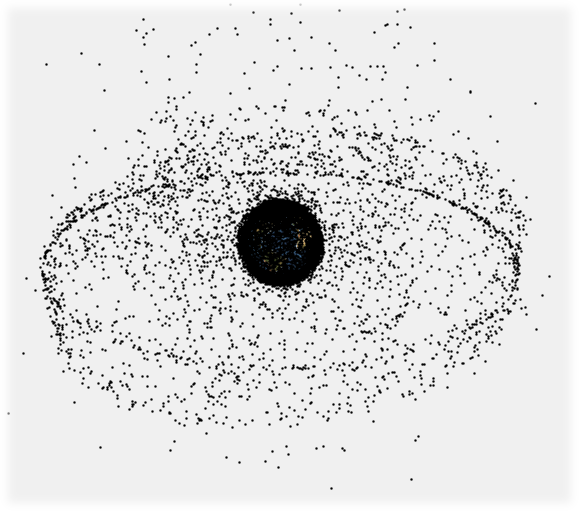
\includegraphics[scale=0.5]{cata2.png}
				\end{figure}
		
		
	%	ince the beginnings of space travel in 1957, the space around our earth has been becoming increasingly congested.
	%	As of 2010 there are over 770 active satellites in either Low Earth Orbits (LEOs), Geostationary Earth Orbits (GEOs) 
	%	or between (Mid Earth Orbits – MEOs) and over 16,000 pieces of catalogued debris larger than 10cm that are being tracked [1]. \newline
	%	In the uncatalogued domain there and millions more objects that have yet to be identified [1]. 
	%	The current overcrowding problem is projected to escalate as additional space missions are launched and as pre-existing debris collides
	%	and shatters, further compounding the problem [2].  
		
		% Image 
		
		In Australia, Optus is responsible for a large portion of the telecommunications infrastructure. According to the Australian Space Environment
		Research Centre (SERC) their fleet of geostationary satellites has a commercial worth of over \$8 billion \cite{SERC}. 
		This entire fleet must be monitored to mitigate risks of collision with debris and avoid loss of assets. \newline
		
		An impact with another orbital object can cause catastrophic damage to an operational satellite, such as shown by the 2009 collision between the 
		active Iridium 33 satellite and the non-operational Kosmos 2251, producing many thousands of pieces of debris larger than 1cm \cite{Kelso}. 
		This debris will continue its orbit for decades to come, as space debris cannot currently be plausibly removed from orbit \cite{Kelso}.
		Thus, Space Situational Awareness (SSA) and Space Surveillance and Tracking (SST) are essential to protecting and maintaining satellite systems. \newline
	
	
	
	
	\chapter{Background}
	
	
	%	You will need to review previous work in the field, which may include
	%	books and papers (``literature''), patents and commercial products
	%	(``prior art''), and earlier work in your Department.  This
	%	information is usually (but not always) collected in a single chapter,
	%	whose title should preferably be more specific and interesting than
	%	the one above.
	
	
	%This format will be discussed in greater detail below.
	
	The following Chapter intends to briefly introduce the broad area of research to which this document relates, as well as cover some of the approaches and technologies used to explore it.
	This chapter will specifically discuss Space Situational Awareness (SSA) and its subsidiary, Space Surveillance and Tracking (SST), representations of uncertainty for orbital objects, and some of the existing technologies which this project will utilise. \newline
	 
		\section{Space Situational Awareness (SSA)}
		
		Space Situational Awareness refers to both the field of study and the ability to track and predict the physical locations of natural and manmade objects in orbit around Earth, with the intention of avoiding collisions. \newline 
		
		SSA has become a significant area of concern due to the increasing quantity of objects in orbit and the increasing investments into and reliance upon satellite technology. \newline
	
	
	

		\section{Space Surveillance and Tracking (SST)}
		
		To attempt to address the massive problem of managing and tracking the countless orbital objects, catalogues of debris fragments, active and inactive satellites are maintained by international agencies. One such database named Celestrak, which is publicly posted and maintained by CSSI (Centre for Space Standards and Innovation), contains an extensive catalogue of NORAD (the North American Aerospace Defense Command) tracked objects stored in a format known as Two-Line Element (or TLE).  \newline
		
		These catalogues can be used to analyse, simulate and predict various future scenarios to assess potential risks to assets. \newline
		
		These simulations and subsequent analysis lead to greater threat identification, preparation and responsive deployment of avoidance measures. \newline
		

		
%		With the sheer numbers of orbit debris objects in the tracking catalogue, it is necessary to filter this catalogue into subsets which can more feasibly be analysed for conjunctions. These subsets can be obtained using geometrical or temporal filters [6]. These subsets can be analysed with root and extrema finding algorithms to isolate time intervals when a pair of elements pass within a specified proximity threshold relative of each other [6]. With this greatly reduced problem space, conjunction analysis can be feasibly carried out on the close proximity pairs [6, 7, 9, 10].
		
		\section{Representations of Uncertainty}
		As with any simulation based on an observation, uncertainty and error of measurements must be considered when analysing simulated results. Traditional analysis of orbital collisions (often referred to as conjunctions) asserts that orbital observation uncertainty will distributed by a Gaussian model. Thus the standard error volume is that of an ellipsoid volume centered on an observation. \newline
		
		This assumption suppresses the true non-Gaussian nature of satellite position uncertainties \cite{Hobson, Ghrist}. A proposed solution for this shortcoming is to treat the non-Gaussian error model as a sum of Gaussian elements, modeling variables such as state noise or measurement noise, which can be assumed to be Gaussian \cite{Jiajun, Terajanu}. This is known as the Gaussian Sum or mixed-Gaussian method. \newline 
		
%		Traditional conjunction analysis uses the assumption that orbital elements will behave according to a roughly Gaussian error model [7, 12, 13]. This assumption supresses .
		
		Similarly, a particle representations can model the non-Gaussian nature of the object. Particle methods utilise Monte Carlo sampling to, effectively, represent uncertainty to a desired level of fidelity based on the number of samples used (where each sample becomes a new 'particle' within a collection). This resulting cloud of particles can then represent the possible states and thus the uncertainty for any orbital object. \cite{Hobson}. \newline
		
		Particle methods are particularly suited to applications with high rates of false detections and extended periods between observations, where a Gaussian-distributed error volume may deviate significantly from the true probability distribution. This point is demonstrated in Fig \ref{guass}, illustrating the discrepancy between a low fidelity Gaussian volume and a higher fidelity particle distribution method. \newline 
		
		\begin{figure}[H]
			\centering
			\caption{Guassian and particle rerpesentations of an orbital object's uncertainty}
			\label{guass}
			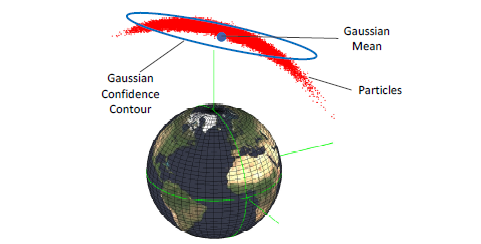
\includegraphics[scale=0.8]{guass.png}
		\end{figure}
		
		Whilst particle methods are significantly more computationally expensive than their Gaussian counterparts, for SSA purposes, the additional fidelity may be desirable.
		
	
		


	
		
		\section{SGP4}
		
		Over 35 years ago, the United States Department of Defense(DoD) released a document SpaceTrack Report Number 3\cite{SpaceTrk3}. Included in this document was the source code used to predict future orbital object positions. The code became known as Simplified
		General Perturbations-4 (SGP4). \newline
		
		 Since the release of this source code, many changes have been made to the official code, which have not been released to the public.Through the many individual efforts from within the scientific community, a non-proprietary version has been created which is highly compatible with its current DoD brethren \cite{SpaceTrk3R}. As of today, SGP4 is available publicly in several coding languages including Fortran, Python, C++ and MATLAB. \newline
		 
		 Using these free software libraries, and using Two-line Element data sets available online, it is possible to predict the future locations of all orbital objects in a given SST catalogue.
		
%		"Over a quarter century ago, the United States Department of Defense (DoD) released the equations and source code used to predict satellite positions through SpaceTrack Report Number 3 (STR#3). Because the DoD's two-line element sets (TLEs) were the only source of orbital data, widely available through NASA, this code became commonplace among users needing accurate results. However, end users made code changes to correct the implementation of the equations and to handle rare cases encountered in operations. These changes migrated into numerous new versions and compiled programs outside the DoD. Changes made to the original STR#3 code have not been released in a comprehensive form to the public, so the code available to the public no longer matches the code used by DoD to produce the TLEs. Fortunately, independent efforts, technical papers, and source code enabled us to synthesize a non-proprietary version which we believe is up-to-date and accurate. This paper provides source code, test cases, results, and analysis of a version of SGP4 theory designed to be highly compatible with recent DoD versions."
		
	
		\section{Two-line Element}
		
		Two-line Element (TLE) is the de facto data representation of an orbital object's Keplerian parameters and is the native data format used with SGP4. The format consists of two lines of ASCII text, each with a length of 70 characters. Some TLE sets contain a title line preceding the TLE data for human readability, but this is not required, as each data line contains a satellite identifier. \newline
		
		Seen in Figure \ref{TLE} below is an example TLE, with the encoding annotated.
		
		\begin{figure}[H]
			\centering
			\caption{Annotated Two-line Element Format, image credit to NASA\cite{NASAtle}}
			\label{TLE}
			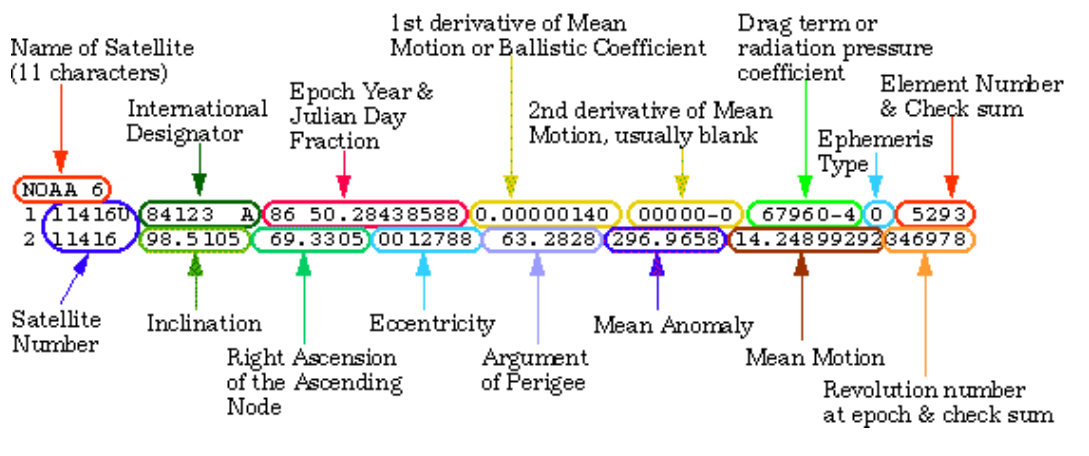
\includegraphics[scale=0.5]{TLE.png}
		\end{figure}
		
		
				
		\section{Existing SSA Visualisations}
		The main proprietary SSA Visualisations are made by Analytical Grapihcs, Inc. (AGI). The only free offering from AGI is the Systems Tool Kit (STK), which has tools for modelling, analysing and visualising time-dynamic positions of objects. \newline
		
		An example visualisation is shown in Figure \ref{AGI}, showing the collision of the active Iridium-33 and inactive Kosmos 2251 satellites on the 10th of February, 2009. \newline

		
			\begin{figure}[H]
				\centering
				\caption{Visualisation of Iridium-33 and Kosmos 2251 Collision using Systems Tool Kit}
				\label{AGI}
				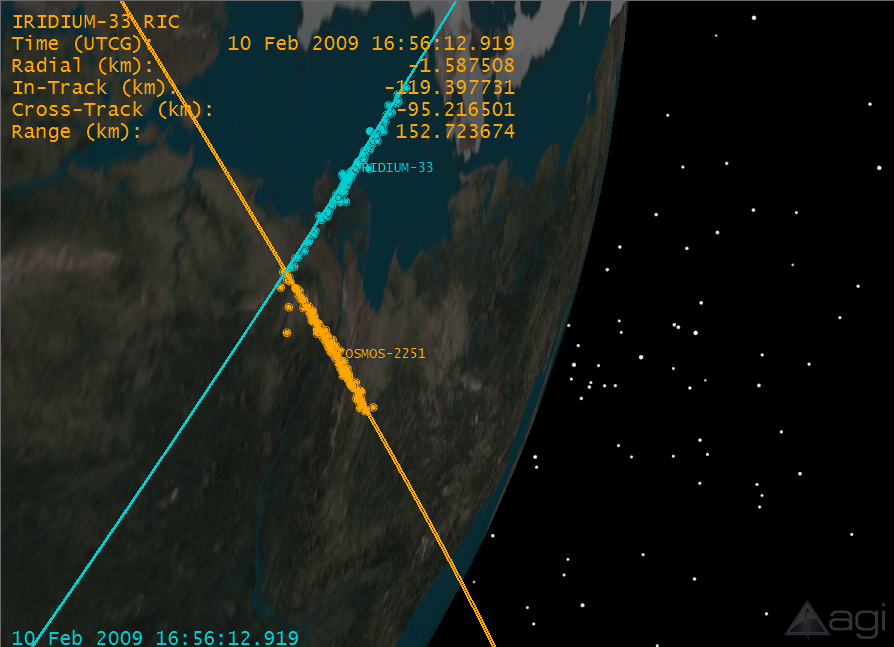
\includegraphics[scale=0.45]{AGI.png}
			\end{figure}
		
		\section{Virtual Reality and HTC vive}
		The recent release of the HTC Vive has enabled interactive Virtual Reality (VR) to be experienced by a wide audience. The HTC Vive itself is a headset and hand-held controller combo that delivers head tracking and stereoscopic 3D visuals on the headset and motion tracking on the wireless controllers.
		
		The most useful quality this experience offers is the immediate impression of scale and presence afforded by the stereoscopic 3D view. The effect itself is profound enough to induce phobias of heights in users \cite{heights}.  \newline
		
		While still a fledgling technology, wide-spread adoption and development by major technology companies has lead to extensive VR support in most major graphics engines. This support, coupled with a booming open source development scene, makes creating VR experiences a fairly approachable endeavor.
		\section{Review}
		
		Within the broad range of aforementioned topics, there is a significant area of investigation encompassing the following:
		
		\begin{itemize}
			\item Investigation of non-Guassian representations of orbital object uncertainty using generative particle methods.
			\item Investigation of the academic applications of cutting edge VR technology to interactive visualisations.
			\item Creation of SSA related visualisations, facilitating further investigation into orbital phenomena.
		\end{itemize}
		
		\section{Thesis Definition and Scope}
		
		Thus, using TLE data from publicly available SST catalogues and the SGP4 propagation model, a visualisation software package will be created to explore the above areas of investigation. \newline
		
		With regards to scope, this thesis will not: 
		\begin{itemize}
			\item Delve deeply into advanced astrophysics theory. It will instead make use of well established astrophysics software libraries in conjunction with sound engineering practices. 
			\item Discuss in rigorous detail the sensor networks that provide the observations contained within the TLE catalogues.
		\end{itemize}
		
		Conversely, this thesis will:
		
		\begin{itemize}
			\item Discuss the engineering practices demonstrated whilst designing,developing and validating the intended visualisation package. 
			\item Discuss the systematic approaches applied in this investigation in response to challenges and problems.
			\item Discuss in detail the above identified areas of investigation, which may be lacking in the current literature.
		\end{itemize}
				
%		Using data from publicly available SST catalogues and a propagation modeller called the Standard General Perturbations Satellite Orbit Model 4 (SGP4) [14, 15] catalogue elements can be propagated forward in time. The standard data format for SGP4 objects is the two-line element set (TLE) which encodes various orbital elements for an Earth-orbiting object for a given moment in time [16]. 
%		AGI, a leading commercial space analytical graphics company is responsible for many software solutions for commercial SSA [17], but these packages are very costly and do not include non-Gaussian collision analysis.
	
%	\chapter{Theory}
%	
%	A scientific paper is likely to be read by people who are not
%	specialists in the same field as the author(s), but who nevertheless
%	may need to use the results of the paper in their own fields.
%	Similarly, the examiners of your thesis will probably include at least
%	one academic who does not teach or conduct research in the subject
%	area of your thesis.  In an early chapter of your thesis, therefore,
%	you should quote any theoretical results which are necessary for the
%	understanding of later chapters.  Examiners who are not specialists in
%	your area will know whether you have given sufficient theoretical
%	information.  They will also know whether you have insulted their
%	status by presenting material which is familiar to every
%	half-competent graduate in every field of ECE.
	
	\chapter{Methodology}
	
	%	This may be one chapter or several.  Again, titles should be more
	%	informative than the above.
	%	
	%	You will almost certainly need diagrams to clarify your meaning.  The
	%	\LaTeXe\ \texttt{graphics} package allows the inclusion of PostScript
	%	graphics, as in \fig{flr1}.  The inclusion of \LaTeX\ \texttt{picture}
	%	graphics, as in \fig{fzsys}, requires no auxiliary packages and allows
	%	the mathematical formatting features of \LaTeX\ to be used in
	%	diagrams; but the \texttt{picture} files, unlike PostScript files,
	%	usually require manual editing.
		\section{Overview}
		There are three seperate programs that were created for this project:
		\begin{itemize}
			\item A simulation and visualisation tool built in MATLAB, which handles the input files and calculation of orbital state vectors at various times and can output to network and to file.
			\item An interactive 3D visualisation built in Unity, which is streamed data from MATLAB and which supports the HTC Vive VR Headset.
			\item An analysis tool built in Java, which reads in data stored in the output files created by the MATLAB component.
		\end{itemize}
%		\subsection{MATLAB}
%		
%		\subsection{Unity}
%		
%		\subsection{Java}
	
		%----------
		\section{Data and Online Catalogues}
		To source TLE datasets, the public catalogue of Two-line Element data sets known as Celestrak was used. Celestrak's primary source of observations is NORAD (the North American Aerospace Defense Command). 		NORAD tracks and maintains TLE sets for all resident space objects over a certain size. \cite{SpaceTrk3} \newline
		
		Similarly, further customised TLE sets can be obtained  from the likewise affiliated online database known as Space Track (after creating an account).
		\cite{spaceTrack}
	
		\section{MATLAB Simulation}
		As discussed above, the MATLAB simulation and visualisation tool reads input TLE set files and calculates future state vectors for each object in the input file. These state vectors are then presented in an animated visualisation, and may be stored in file or sent over network. \newline 
		
		
		Thus, the tasks handled by the MATLAB program can be broken down into the following:
		\begin{itemize}
			\item TLE Reading
			\item Particle Generation
			\item SGP4 Propagation
			\item MATLAB Visualisation
			\item Output to file / network
		\end{itemize}
		\subsection{TLE File Handling}
		Using the Celestrak database, TLE datasets can be downloaded and stored in plain text files. Processing of these plain text files with TLE data is a matter of reading each line and storing these lines, to be later processed. The file handling routine can be found in Appendix A.1. \newline
		
		
		These lines are later processed through the the \texttt{tleToSatrec} routine, which creates a structure data type 'satrec' which contains the contents of the TLE file seperated into their respective fields. Usage for this routine is as follows: \newline
		
		[satrec] = \textbf{tleToSatrecO}(\textit{gravConst, line1, line2, runType, typeInput, startmfe, stopmfe, deltamin}) \newline
	
		Where \textbf{gravConst} is the gravity constant used (from a selection of constants of varying fidelity), \newline 
		\textbf{line1} and \textbf{line2} are the TLE lines \newline
		\textbf{runType} and \textbf{typeInput} are various methods within SGP4 (manual mode 'm' and a customised input 'j' were used)\newline
		The \textbf{startmfe} and \textbf{stopmfe} are the supplied start and stop times \newline
		And \textbf{deltamin} is timestep value.
		
		\subsection{Particle Generation}
		Particles, $p^r$, are generated by adding a noise vector $\phi^r$ (modeling the error as per \cite{Hobson}), to their  initial state $x_i$ , read from the TLE. This can be seen in equation:
		\begin{equation}
		p_r = x_i + \phi_r 
		\end{equation}
		Where $\phi_r$ is the noise vector defined as
		\begin{equation}
		\phi_r \sim N(0, \gamma_r^2); \gamma_r^2 = diag \begin{bmatrix} 0.0005\degs \\ 0.0005\degs\\ 0.00001\\
		0.0005\degs\\ 0.00001\degs\\ 0.00001 orbits/day \end{bmatrix}
		\end{equation}
		
		This above noise / error vector was used in \cite{Hobson}, found empirically to model appropriate levels of perturbations experienced by orbital objects.
%		\begin{flushright}
%			
%		\end{flushright}


		All particles are then propagated forward in time using the SGP4 model.
		
		The full particle generation routine, which is tied to the tleToSatrec routine detailed above can be found in Appendix A.2.
		\subsection{SGP4 Propogation}
		
		Now that the \textbf{satrec} structure has been created for each object, \textbf{satrec} can be passed to the \textbf{sgp4} function, along with the time (measured in Julian Days) at which to calculate the state vectors of the object. This is performed for every particle of every object, at every desired time. These results can then be visualised. \newline 
		
		To improve performance, these routines were adapted for parallel computation and performed on the GPU via nVidia's CUDA environment within MATLAB's Parallel Computing Toolbox. This will be discussed further in the GPU Parallelism Section \ref{gpuPerf}. Furthermore, due to the large number of calls to these routines, they were optimised slightly by replacing computationally expensive operations such as multiplication and squaring with pre-computed constants where possible. \newline
		
		\subsection{Visualisation}
		
		Using the MATLAB built-in plotting function \textbf{scatter3} (the 3D variant of the \textbf{scatter} plot function), alongside a textured 3D mesh of the earth, a snapshot of the locations of all the input orbital objects can be visualised. This is achieved with the following psuedocode:
				
		\begin{algorithm}[H]
			\caption{Built-in MATLAB visualisation Pseudocode Snippet}
			\label{visM}
			Where $o$ is an abritrary orbital object, $S$ is the set of all objects in the input dataset \newline
			
			xArray = xComponent $\forall o \in S$ \newline
			yArray = yComponent $\forall o \in S$ \newline
			zArray = zComponent $\forall o \in S$ \newline
			
			hold on \newline
			
			scatter3(xArray, yArray, zArray) \newline
			
			eTex = imread('earthmap.jpg') \newline
			[x1, y1, z1] = sphere(100) \newline
			earth = surf(x1*6000,y1*6000,z1*6000, 'EdgeColor','none') \newline
			set(earth,'CData',flipud(eTex),'FaceColor', 'texturemap') \newline
			
			cameraInit(angles)
		\end{algorithm}
		 
		 This static visualisation can then be animated by sequentially changing the supplied position arrays for each frame, at some arbitrary rate of frames per second (frame rate of animation). \newline
		 
		 This is achieved with the MATLAB built-in \textbf{set} which allows a plot to be supplied new data, \textbf{drawnow} which updates the rendered plot, and \textbf{pause} which pauses for a time measured in seconds. \newline
		 
		 Algorithm \ref{visM} is extended with the following to achieve an animated visualisation:
		
				\begin{algorithm}[H]
					\caption{Built-in MATLAB Animation Pseudocode Snippet}
					\label{aniM}
					Where $o$ is an arbitrary orbital object, $S$ is the set of all objects in the input dataset \newline
					\begin{algorithmic}
						

					\While{Animating}
						
						\State tic (begin timing) \newline
						
						\State xArray = nextXComponent $\forall o \in S$
						\State yArray = nextYComponent $\forall o \in S$
						\State zArray = nextZComponent $\forall o \in S$ \newline 
						
						\State h = reference to scatter plot \newline
						
				    	\State set(h, 'xdata', xArray, 'ydata', yArray, 'zdata', zArray)
				    	\State drawnow
				    	\State toc (take a measurement of the elapsed time since tic was called)\newline
					    
				        \State pause(1/fps-toc)
				    \EndWhile
     				\end{algorithmic}

				\end{algorithm}
		
		\subsection{UDP Communication}
		
		Using the built-in \textbf{UDPSender} object from the MATLAB Digital Signal Processing Toolkit (installed by default),
		data can be sent over User Datagram Protocol (or UDP), facilitating real-time communication between programs either locally or over network. \newline 
		
		UDP was chosen over TCP/IP to minimise network overhead and because packet loss was desirable over waiting for delayed packets. \newline
		
		The \textbf{UDPSender} object was chosen over the alternative MATLAB \textbf{udp} object, for it's maximum output buffer size (twice that of \textbf{udp})). \newline
		
		Usage within MATLAB is as follows:
		
		\begin{itemize}
			\item Initialise destination with \textbf{UDPSender} object.
			\item Explicitly convert data to be sent into a binary format (e.g using \textbf{int16} or \textbf{int32}).
			\item Send the data through the UDPSender object using the function \textbf{step}.
			\item Release the UDPSender object using \textbf{release} (allowing different format data to be sent).
		\end{itemize}
		
		In pseudocode, this is: 
		
		\begin{algorithm}[H]
			\caption{MATLAB UDP Psuedocode}
			\label{aniM}
			Where $objs$ is the data object to be sent\newline
			\begin{algorithmic}
				
				
				\State hudps = dsp.UDPSender(RemoteIPAddress, RemoteIPPort)
				
				\State data = convert $objs$ to desired binary representation (i.e. int16(objs))
				\State step(hudps,data)
				\State release(hudps)

			\end{algorithmic}
			
		\end{algorithm}
%		\begin{figure}[H]
%			\centering
%			\caption{MATLAB UDP Code Snippet}
%			\label{AGI}
%			\includegraphics[scale=0.8]{UDPsnippet.png}
%		\end{figure}
		
		
		\section{GPU Parallelism}
		With the set goal of creating a real time visualisation, the problem of computing computationally intensive routines for a large dataset was a significant technical challenge. Fortunately, the computation of each object is independent and thus can be calculated in parallel (or as close to parallel as the computation hardware would allow). \newline
		
		Thus, using nVidia's CUDA Parallel Programming environment and a low-end nVidia card, these independent operations can be paralellised, contributing to a considerable speedup. Thanks to support for CUDA within MATLAB's Parallel Computing Toolbox, this parallelisation can be accomplished mostly within MATLAB by adapting the existing code. \newline
		
		The primary chunk of code to parallelise was the SGP4 routine for each object. This meant performing both the SGP4 initialisation (sgp4init)and the SGP4 propagation function (sgp4) for each timestep for each object on the GPU. \newline
		
		Thus, the steps needed to parallelise the code were as follows:
		
		\begin{itemize}
			\item Adapt the SGP4 code to the programming language C. Fortunately, a version of SGP4 already exists written in C, which was used.
			\item Split the GPU up into blocks upon which the parallel calls can be processed.
			\item Write the CUDA function to run the sgp4init and sgp4 for each object and timestep in using the above blocks. This CUDA function can be called from within MATLAB.
			\item Pass the GPU the data structure \textbf{satrec} for each object. Since passing data structures between languages is messy, the required contents of the data structures were passed as flat arrays with the index of the array corresponding to an object.
			\item Retrieve the results from the GPU, stored in a flat array storing the x,y and z components of each object.
		\end{itemize}
		
		The MATLAB code snippets implementing this can be found in Appendix A, Figure A.3, and the CUDA code can be found in Appendix A, Figure A.4. \newline
		
		With the speedups afforded by the above parallelisation(for full speedup data, refer to the Section \ref{gpuPerf}), the MATLAB visualisation moved from a strategy of "pre-compute, then display results sequentially" to a strategy of "compute once every \textbf{X} frames, then display those \textbf{X} frames", thus allowing an endless, real time visualisation. The strategy of computing \textbf{X} frames is to minimise delays due to computation.
		
		\section{Unity Visualisation}
		
		To overcome the constraints of the MATLAB visualisation, a companion visualisation was built in Unity. The allowed greater control over all aspects of the visualisation but primarily relating to the graphics pipeline, camera control and user interactivity. \newline
%		Due to the constraints of the MATLAB visualisation
		
		\subsection{Receiving Data over UDP}
		Using the above methods to send data to a remote IP Address and port via UDP, position data for each frame was able to be sent from an instance of MATLAB to an instance of Unity. This data was received and processed in a separate 'slave' thread. \newline 
		
		During the initialisation of communications, the total number of objects (inclusive of the number of particles for each object) is sent by from MATLAB and stored by Unity. After this number has been stored, the master thread instantiates that many objects and stores a reference to them. \newline
		
		All future communications are then expected to be frame updates. Each frame update is then decoded and stored in a queue accessible by the main thread. Code snippets of this routine can be found in Appendix Figure A.5.\newline

		\subsection{Animation}
		Using the built-in Unity function \textbf{Update()} which is by default called before every frame rendered in Unity, if the MATLAB frame queue is not empty, the top most entry is popped from the queue and processed. \newline
		
		This processing reads the changes for each object from the entry and updates the corresponding the position vector for each object, using the reference instantiated on initialisation. 
		
		\subsection{Virtual Reality with HTC Vive}
		Thanks to the design of plugins within Unity, adding support for Virtual Reality within Unity is a trivial task. The primary plugin used was SteamVR which assists in connecting a Unity instance to an local instance of Steam (a software distribution platform), which acts as a hub or 'menu' for the VR device (HTC Vive in this case). 
		\subsubsection{SteamVR}
		
		Using the aforementioned SteamVR plugin, synchronising the visualisation camera and the VR headset is as simple as adding a prefab asset (a predefined entity) into the Unity environment. This asset also gives access to controller inputs which can be coded to provide interaction. In this project, controller interaction was limited to teleportation movement.
				
		\subsubsection{Teleportation}
		Using a modified open source framework, the HTC Vive controllers were configured to allow the user to teleport around the 3D environment. This was an extension of the real movement of the user in the real room, which is a bounded area. With the teleportation implementation, the user is able to move where the bounded area is in the digital space. This has become somewhat of a widely adopted method of locomotion in VR simulations, as automatic or guided locomotion can induce motion-sickness in users. \newline
		
		Working in tandem with this script was an invisible 2D plane running through with centre of the earth and covering the entire environment, which acts as the collision plane (the area to which the player may teleport). \newline
		
		\textbf{PLEASE NOTE:} the implementation of this script is not the author's work and full credit for this open source framework is given to the rightful creator \cite{tele}. \newline
		
		With the above implementations, the Unity visualisation was enhanced by the perception of real movement within the digital environment and stereoscopic 3D.
		
		
		\section{Close Approach Analyser}
		
		To avoid hindering the performance of either the MATLAB or Unity visualisations, it was decided to build the analysis tool separately, as a companion tool to be used post-simulation. This goal of this tool was to use the propagated position information from the MATLAB simulation to perform calculations as to the chance of any collisions between every unique pairing of objects (and particles not of the same object). \newline
		
		Due to the author's comfort with the Java language, it was chosen to quickly build the analysis tool. This brough the total programming language count used in this project up to four. \newline
		
		Using the output files created by the MATLAB simulation (containing all propagated particles and objects at all timesteps the simulation calculated) as the input for this tool, each time-step was checked for close approaches by comparing comparing the close approach threshold radius to the distance calculated using the Euclidean distance formula: \newline

		For two points $P_1 = (x_1, y_1, z_1), P_2 = (x_2, y_2, z_2)$, \newline
		
		\begin{equation}
			D(P_1, P_2) = \sqrt{(x_1-x_2)^2 + (y_1-y_2)^2 + (z_1-z_2)^2}
		\end{equation} \newline
		
		
		Initially, the close approach threshold radius was an estimate of the average size of a satellite, but this was recognised as a naive approach, as the fidelity required for this calculation to be valid was completely unfeasbile. Thus the close approach threshold radius was set between 15 and 30km. This value was chosen based on the age of the TLE file used. The age of a TLE file can be found by taking the difference between the simulation time and the time since the epoch (reference date) of the TLE. \newline
		
		The close approach threshold range of 15-30km was reasoned as appropriate, given the estimated accuracy of an average 3 day old TLE set is 30km \cite{agiAcc}. It is worth noting that accuracy of TLE sets have been found to vary wildly from source to source, with some sources having accuracy down to 1km at epoch and as high as 300km at epoch. Historically, TLE's have been shown to occasionally exceed the characteristicly estimated accuracy by a factor of twenty when compared to positionally well-known satellites (e.g. tracked by GPS). \cite{agiTLEAcc}. \newline
		

	
	
	% --------------------------- %
	\chapter{Results}
	
	Links to videos of both the MALTAB and Unity visualisations as well as source code can be found in Appendix B.
	
		\section{MATLAB Visualisation}
		
		A number of visualisations of different catalogues with various configurations of particles will be shown. The various catalogues correspond to different groupings of objects, grouped by orbit classifcation. These orbits are introduced without particles showing error, and then with particles to demonstrate the uncertainty in each catalogue. Note the along-track variance (variance in distance along the direction of the velocity vector). 
		
		\subsection{Catalogue Visualisations without Particle Generation}
		
		The following figures show snapshots of various TLE catalogues visualised without particle clouds representing uncertainty volumes. Figure \ref{cata2} seen below shows the current complete catalogue of 15500 objects being tracked.
		

			\begin{figure}[H]
				\centering
				\caption{MATLAB Visualisation of 'Complete' TLE Catalogue}
				\label{cata2}
				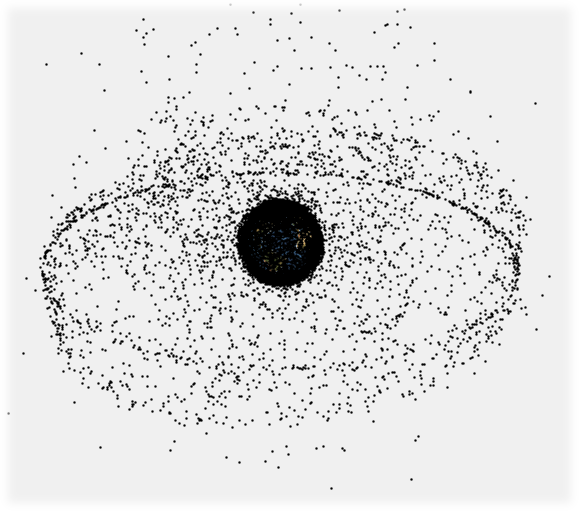
\includegraphics[scale=0.5]{cata2.png}
			\end{figure}
			
			\begin{figure}[H]
				\centering
				\caption{MATLAB Visualisation of Low Earth Orbit Catalogue}
				\label{LEO}
				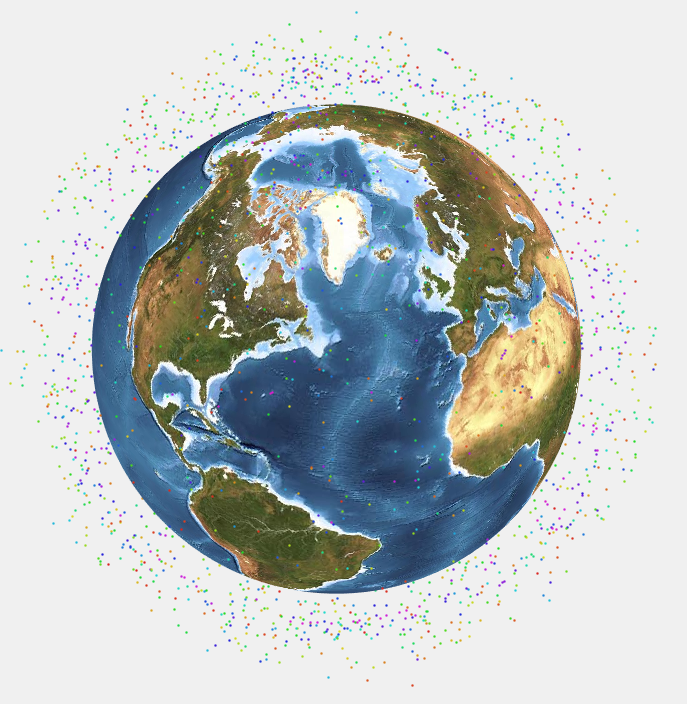
\includegraphics[scale=0.6]{LEO.png}
			\end{figure}

			\begin{figure}[H]
				\centering
				\caption{MATLAB Visualisation of Highly Elliptical Orbit Catalogue}
				\label{HEO}
				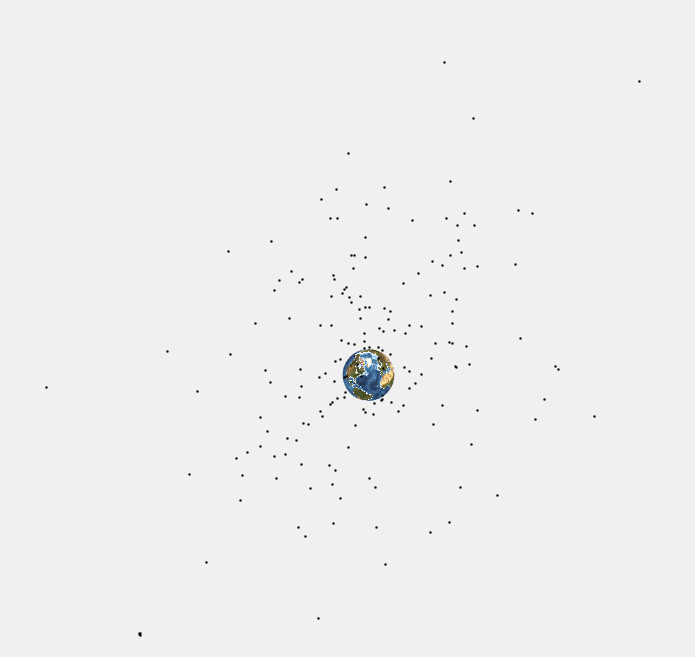
\includegraphics[scale=0.6]{HEO.png}
			\end{figure}
			
			\begin{figure}[H]
				\centering
				\caption{MATLAB Visualisation of Medium Earth Orbit Catalogue}
				\label{MEO}
				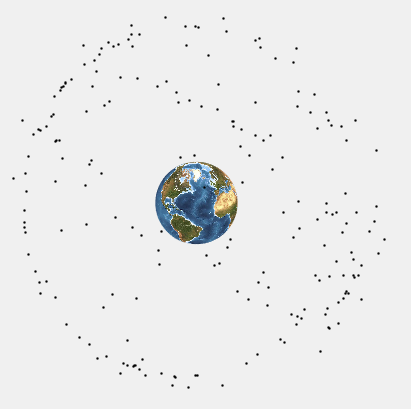
\includegraphics[scale=0.8]{MEO.png}
			\end{figure}
			
			\begin{figure}[H]
				\centering
				\caption{MATLAB Visualisation of Geosynchronous Earth Orbit Catalogue}
				\label{GEO}
				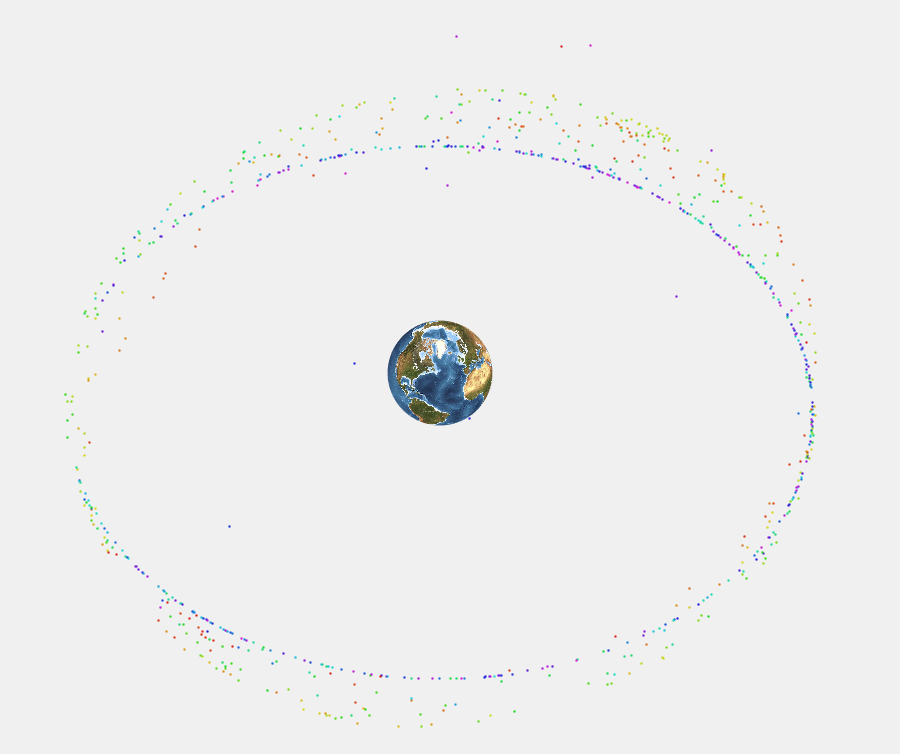
\includegraphics[scale=0.6]{GEO.png}
			\end{figure}

		\subsection{Particle Generation}
		
		The following visualisations show snapshots of various TLE catalogues visualised with particle clouds of size 100. It is important to note a higher particle count is often required to accurately represent error for analysis purposes, but for visualisation purposes, 100 is sufficient. Unless stated otherwise, all visualisations used the most recent possible TLE set at the time of visualisation, sourced from Space-Track. \newline
		
		Each particle cloud for each object is coloured the same, although due to the large number of objects, colours had to be re-used. \newline
		
		Note that despite using the most recent TLE sets (less than a day old) the particle clouds had substantial along-track uncertainty (on average $\pm$250km for Low Earth Orbit).
	
				\begin{table}[H]
					\caption{Average along track uncertainty}
					\centering
					\begin{tabular}{ll}
						\toprule
						%\multicolumn{2}{r}{} \\
						Catalogue & Uncertainty \\
						\midrule
						LEO & $\pm250km$ \\
						MEO & $\pm1200km$  \\
						HEO & $\pm1900km$ \\
						GEO & $\pm2400km$ \\
						\bottomrule
					\end{tabular}
				\end{table}	

			\begin{figure}[H]
				\centering
				\caption{MATLAB Visualisation of Low Earth Orbit Catalogue with 100 particles/object}
				\label{cLEO}
				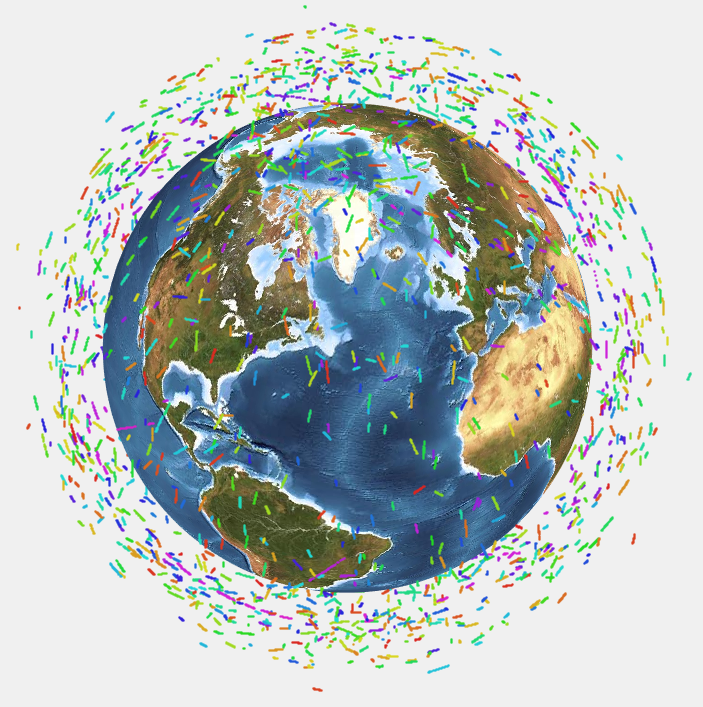
\includegraphics[scale=0.45]{p100LEO.png}
			\end{figure}

			\begin{figure}[H]
				\centering
				\caption{MATLAB Visualisation of Medium Earth Orbit Catalogue with 100 particles/object}
				\label{cMEO}
				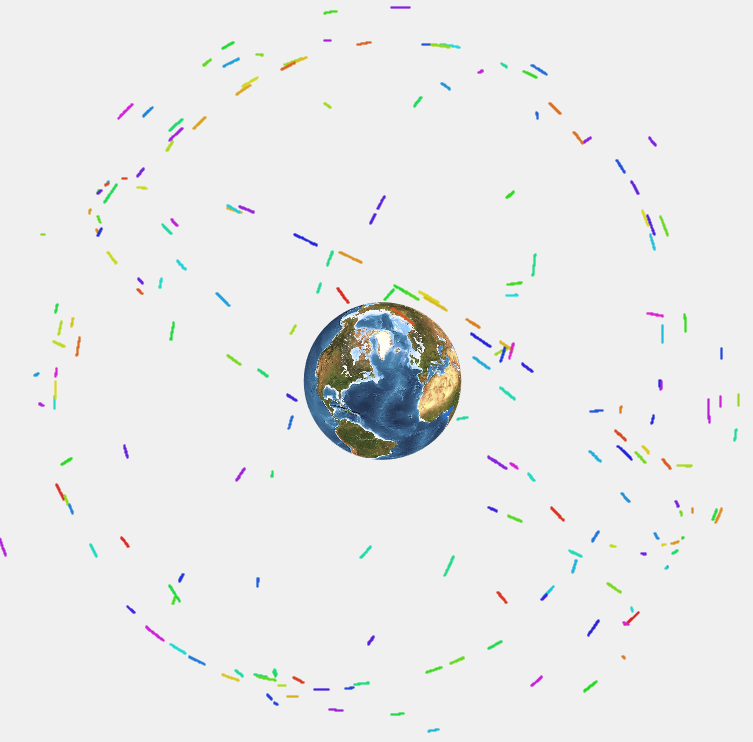
\includegraphics[scale=0.5]{c100MEO.png}
			\end{figure}
			
			\begin{figure}[H]
				\centering
				\caption{MATLAB Visualisation of Highly Elliptical Orbit Catalogue with 100 particles/object}
				\label{cHEO}
				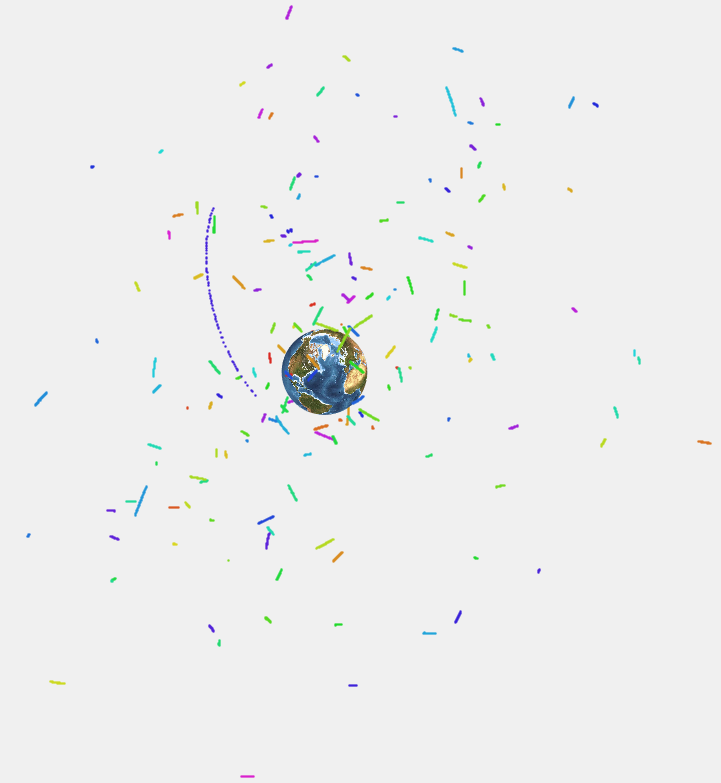
\includegraphics[scale=0.5]{c100HEO.png}
			\end{figure}
			
			\begin{figure}[H]
				\centering
				\caption{MATLAB Visualisation of Geosynchronous Earth Orbit Catalogue with 100 particles/object}
				\label{cGEO}
				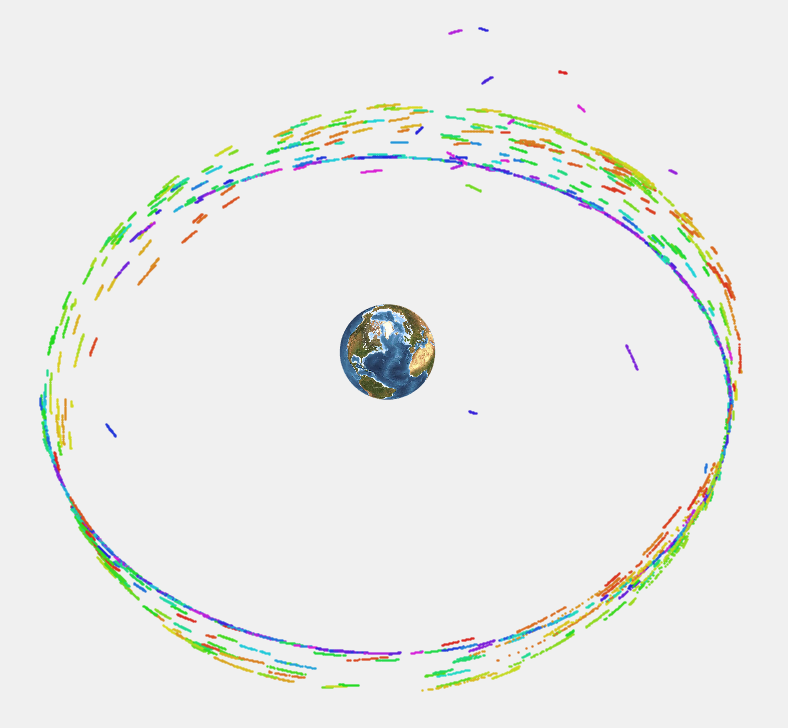
\includegraphics[scale=0.5]{p100GEO.png}
			\end{figure}
			
			\begin{figure}[H]
				\centering
				\caption{MATLAB Visualisation of Orbital Communications Catalogue with 100 particles/object}
				\label{cComms}
				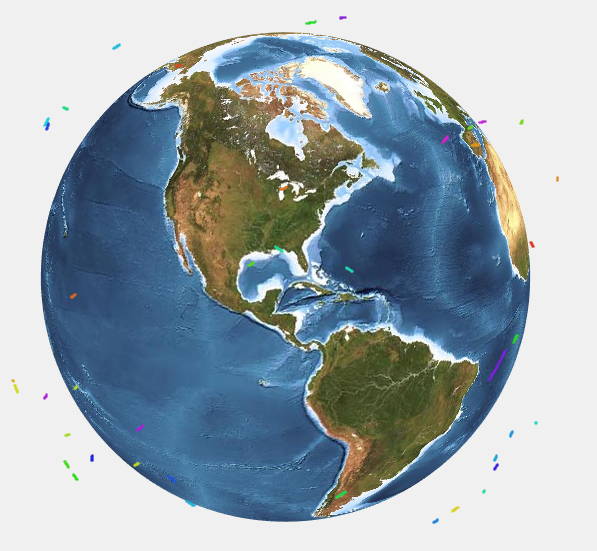
\includegraphics[scale=0.6]{p100Comm.png}
			\end{figure}
		
		\section{Unity Visualisation}
		
		The following figures show Unity visualisations of various catalogues.
		
				\begin{figure}[H]
					\centering
					\caption{Unity Visualisation of Low Earth Orbit Catalogue (verifcation)}
					\label{unityLEO}
					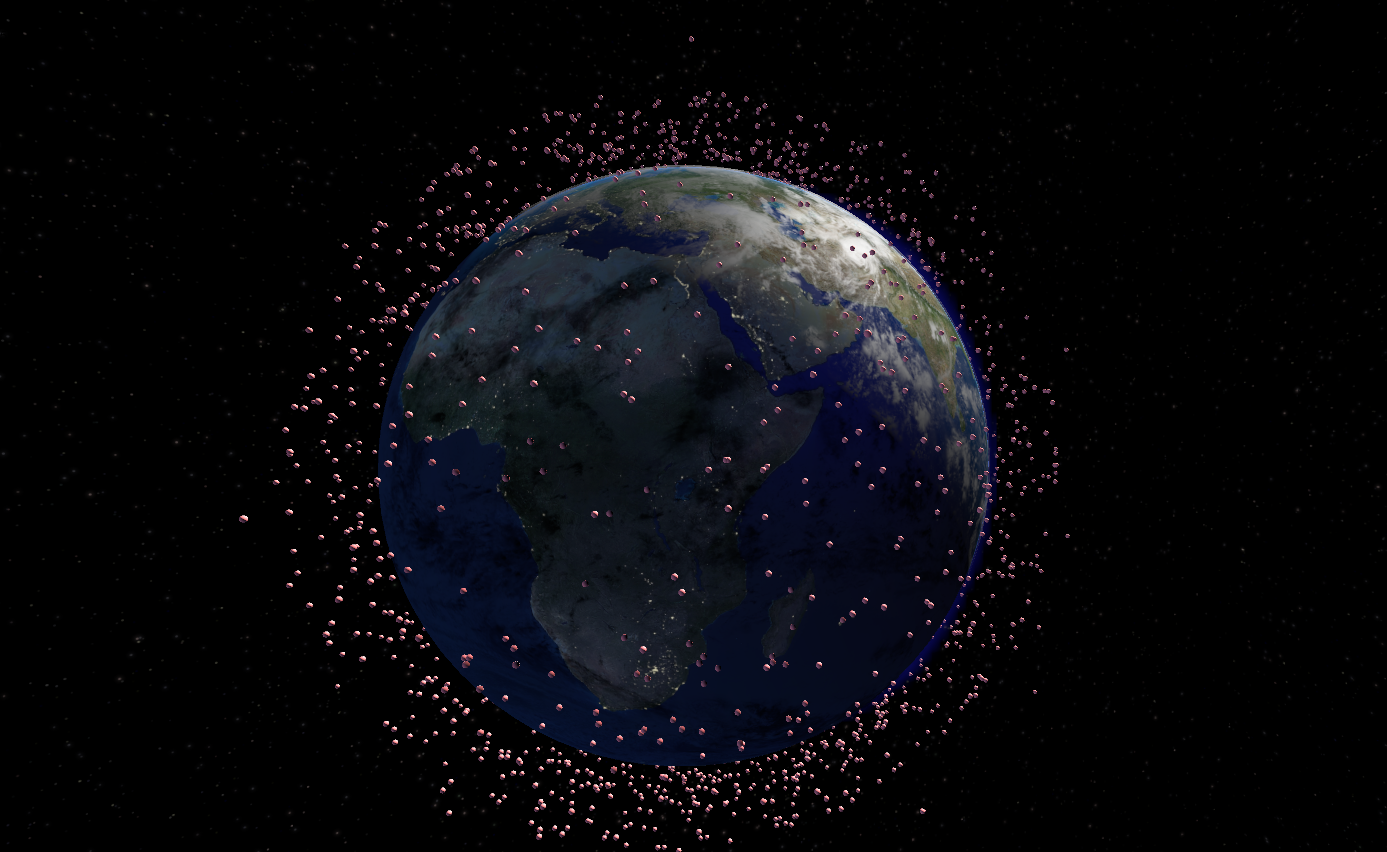
\includegraphics[scale=0.4]{uLEO.png}
				\end{figure}
				
				\begin{figure}[H]
					\centering
					\caption{Unity Visualisation of two week old TLE set with 400 particles/object, showing TLE accuracy decay}
					\label{unityOutD}
					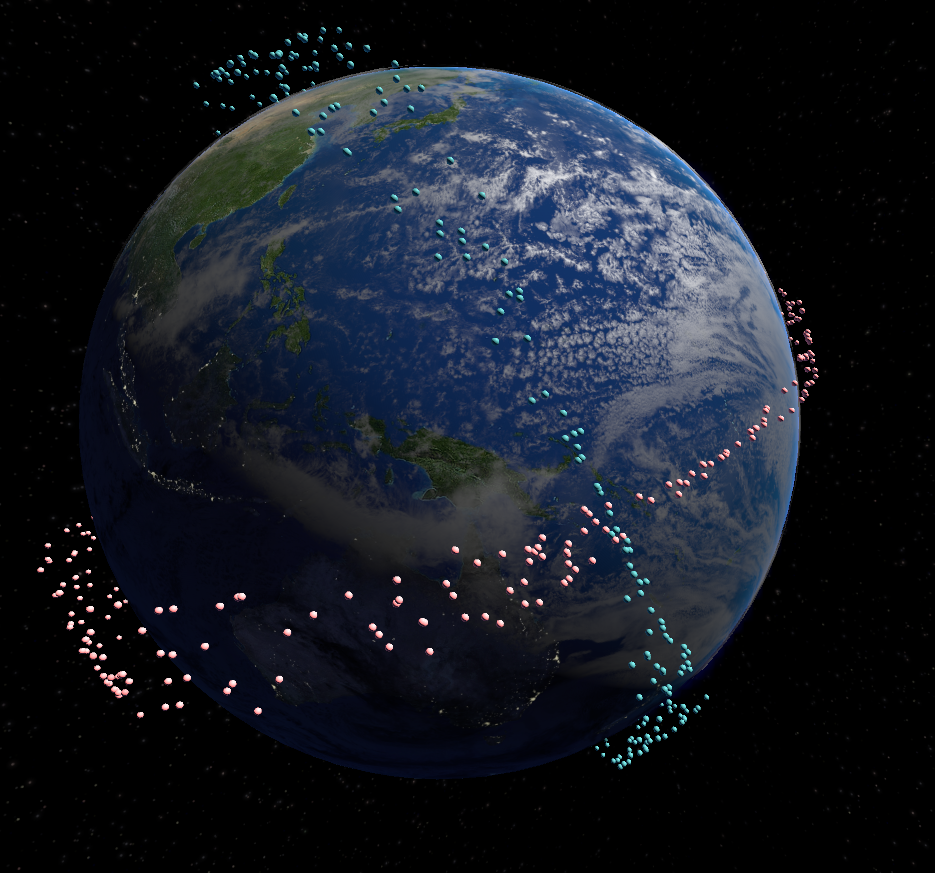
\includegraphics[scale=0.4]{unityOutD.png}
				\end{figure}
				

				
				\begin{figure}[H]
					\centering
					\caption{Unity Visualisation of Highly Elliptical Orbit Catalogue with 25 particles/object}
					\label{unityHEO}
					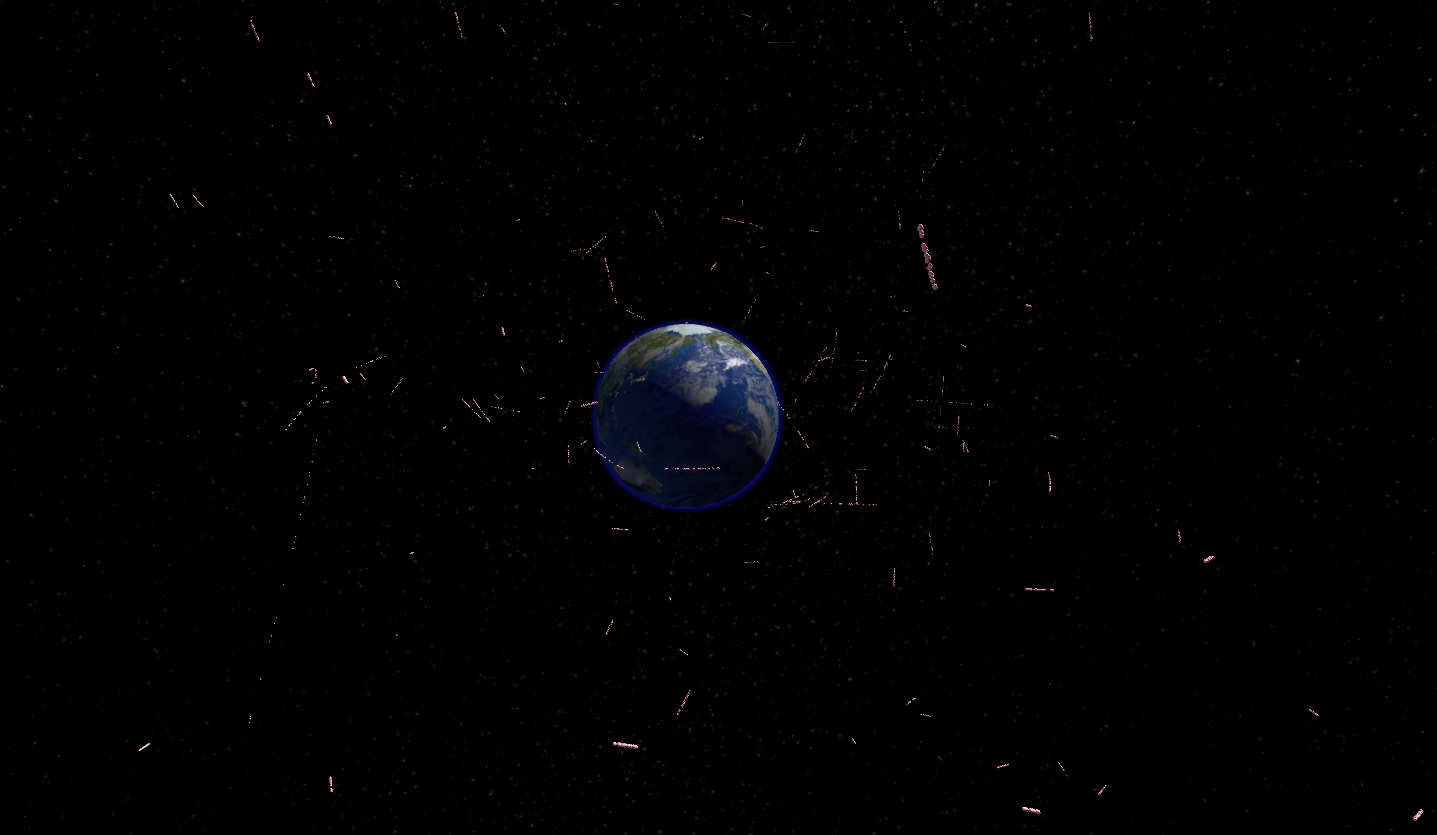
\includegraphics[scale=0.45]{uHEO.png}
				\end{figure}
				
				\begin{figure}[H]
					\centering
					\caption{Unity Visualisation of Medium Earth Orbit Catalogue with 25 particles/object}
					\label{unityMEO}
					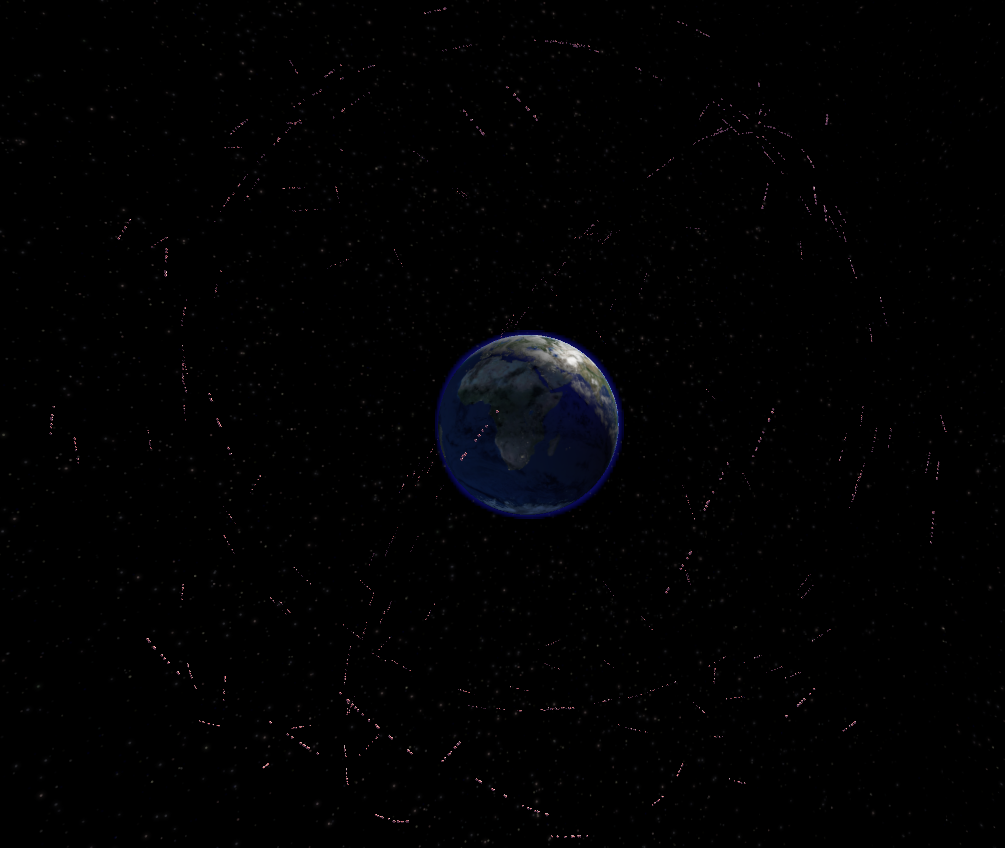
\includegraphics[scale=0.55]{uMEO.png}
				\end{figure}
				Figure \ref{unityTele} shows the teleportation movement indicator, demonstrating where the user will teleport to when they release the trigger input. 
				\begin{figure}[H]
					\centering
					\caption{Unity Teleportation shown in text environment, allowing movement outside of room bounds, using framework from \cite{tele}}
					\label{unityTele}
					\includegraphics[scale=0.5]{telescript.png}
				\end{figure}

		%----------
		\section{GPU Parallelism Performance}
		\label{gpuPerf}
		After parallelising the propagation code, the computation time for the parallel implementation was compared with the serial implementation for various numbers of objects and frames to compute. The results are shown below.
		
			\begin{table}[H]
				\caption{Average computation time of serial and parallel implementation for 1 frame for varying numbers of objects}
				\centering
				\begin{tabular}{llr}
					\toprule
					\multicolumn{3}{r}{Average Run Time} \\
					\cmidrule(r){2-3}
					Num. Objects & Serial & Parallel \\
					\midrule
					15500 & $102s$ & $13.1s$ \\
					2200 & $4.30s$  & $1.70s$ \\
					333 & $0.69s$ & $0.29s$ \\
					24 & $0.13s$ & $0.05s$ \\
					
					
					%\bottomrule
				\end{tabular}
			\end{table}	
		
		\begin{table}[H]
			\caption{Average computation time of serial and parallel implementation for 100 frames for varying numbers of objects}
			\centering
			\begin{tabular}{llr}
				\toprule
				\multicolumn{3}{r}{Average Run Time} \\
				\cmidrule(r){2-3}
				Num. Objects & Serial & Parallel \\
				\midrule
				15500 & $145s$ & $16.0s$ \\
				2200 & $32.0s$  & $1.70s$ \\
				333 & $0.96s$ & $0.30s$ \\
				24 & $0.15s$ & $0.05s$ \\

				
				%\bottomrule
			\end{tabular}
		\end{table}	
		
		\begin{table}[H]
			\caption{Average computation time of serial and parallel implementation for 1000 frames for varying numbers of objects}
			\centering
			\begin{tabular}{llr}
				\toprule
				\multicolumn{3}{r}{Average Run Time} \\
				\cmidrule(r){2-3}
				Num. Objects & Serial & Parallel \\
				\midrule
				15500 & $1422s$ &  N/A (Out of VRAM) \\
				2200 & $176s$  & $3.00s$ \\
				333 & $26.8s$ & $0.41s$ \\
				24 & $1.99s$ & $0.06s$ \\
				
				
				%\bottomrule
			\end{tabular}
		\end{table}	
		
		\begin{figure}[H]
			\centering
			\caption{Average Compute Time vs Number of Objects for 100 Frames}
			\label{perfSer}
			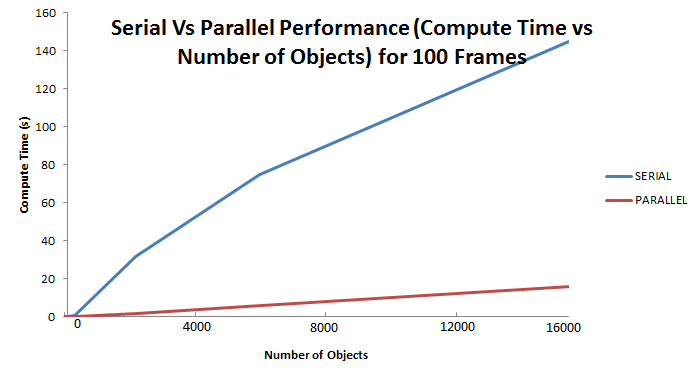
\includegraphics[scale=0.7]{perfSer.png}
		\end{figure}
		
		\begin{figure}[H]
			\centering
			\caption{Speedup Factor from Parallel to Serial Implementation for 100 frames}
			\label{speedup}
			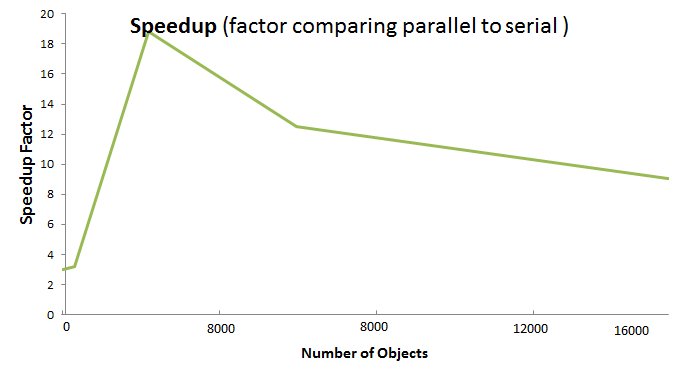
\includegraphics[scale=0.7]{speedup.png}
		\end{figure}
		
		\begin{figure}[H]
			\centering
			\caption{Average Compute Time vs Number of Objects for 1000 Frames}
			\label{perf1000}
			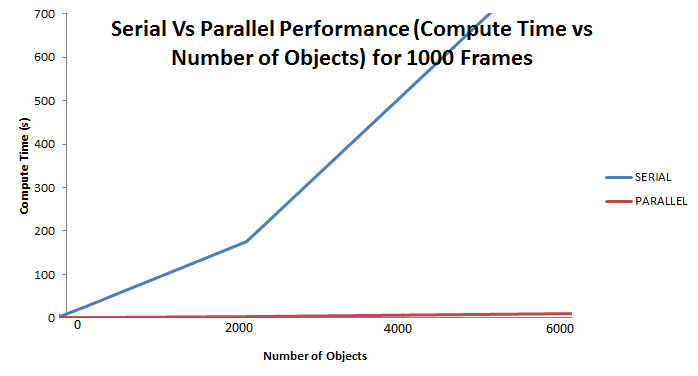
\includegraphics[scale=0.7]{perf1000.png}
		\end{figure}
		
		\begin{figure}[H]
			\centering
			\caption{Speedup Factor from Parallel to Serial Implementation for 1000 frames}
			\label{speedup1000}
			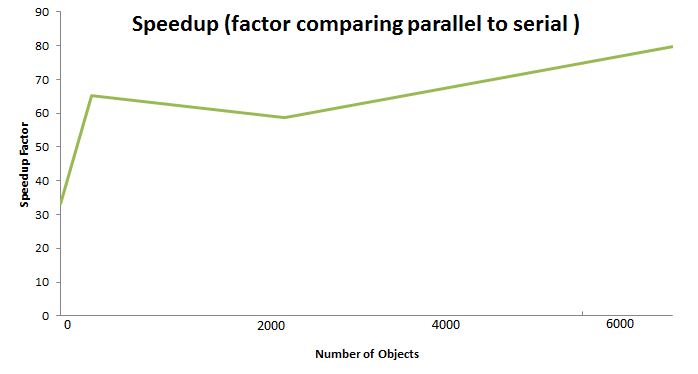
\includegraphics[scale=0.7]{speedup1000.png}
		\end{figure}
		

		
		
		\section{Close Approach Analyser}
		
		To test the close approach analyser, the analysis tool was run using a TLE set with a known collision. The chosen collision was the Iridium 33 and Kosmos 2251 collision on February 10, 2009, at 16:56 UTC, with a TLE containing those two satellites with an epoch at 16:50 UTC. \newline
		
		This TLE is then run through the MATLAB Simulation with 20,000 particles, until the collision is visually confirmed. The simulation can then exit, and the output file created will contain all of the positions of all 20,000 particles for both satellites, at all timesteps (from 16:50 UTC to approx 16:57 UTC in 0.1 minute timesteps). \newline
		
		This output file is then input into the analysis tool which will give the probability of a close approach (which is the fraction of all particles that experienced a close approach). \newline
		
		This analysis was performed at varying close approach thresholds, and the results can be seen below in Table \ref{closeApp}.
		
				\begin{table}[H]
					\caption{Probability of close approach for varying threshold}
					\label{closeApp}
					\centering
					\begin{tabular}{ll}
						\toprule
						%\multicolumn{2}{r}{} \\
						Threshold & Probability \\
						\midrule
						15km & $0.15$ \\
						20km & $0.512$  \\
						25km & $0.831$ \\
						\bottomrule
					\end{tabular}
				\end{table}	
				
		

%	\ldots\ or perhaps the discussion should be a separate chapter.
%	
%	In any case, you will probably need to include tabulated results.
%	\tab{tf2} illustrates the use of various \LaTeX\ environments to
%	include a computer printout (plain text file) in a document.  The
%	\texttt{verbatim} environment, which encloses the formatted text, is
%	also useful for program listings.
	

	
	\chapter{Discussion}
	
	\section{Particles}
	The most significant result of the investigation with respect to the use of particles instead of Gaussian volumes, was the significant along track uncertainty observed, even close to epoch. The comparatively minimal across track uncertainty and curvature of the observed particle cloud further supports the theory of significant discrepancies between the true distribution of error and that represented with an ellipsoid volume. This supports the use of particle representations of uncertainty over Gaussian volumes with TLE analysis. \newline
	
	Further investigation directly comparing the impact of inaccuracy in Gaussian error volumes with Monte-Carlo particle representations in the context of low fidelity threat detection such as those described in this document is needed to quantify this relationship.
	
	\section{Parallelisation}
	
	Due to the independent nature of each object within a large set of objects, the problem was highly parallelisable, with speedups of up to 80 times observed, using a low-end graphics card. This significant speedup was a result of unnecessarily sequential operations being parallelised. \newline
	
	Use of a graphics card with more VRAM would allow larger problems to be simulated and also allow greater parallelisation, assuming transfer speeds to and from the GPU did not quickly become a bottleneck for performance. \newline
	
	This intrinsic affinity for parallelisation supports the effectiveness of supercomputer/cluster approaches to simulating large catalogues of objects with massive numbers of particles.
	
	\section{UDP Bottleneck}
	
	Communications between MATLAB and Unity over UDP was a significant bottleneck due to the large amounts of data being sent. If all objects were sent as an individual message, performance on the receiving end in Unity was poor. Conversely, sending all objects as one message improved performance, but imposed a cap on the number of objects that could be sent, due to the native implementation of UDP communications in MATLAB having an output buffer size of 8192 bytes. Fortunately, the number of objects required to hit this cap was similar to the number of objects required to hit a performance cap with significant slowdowns. \newline 
	
	Thus, if the Unity visualisation was to be optimised further, the following areas would need to be addressed:
	
	\begin{itemize}
		\item MATLAB output buffer size problem. This could be bypassed by sending chunked data when this output buffer size is reached, or by writing a new UDP implementation with a larger output buffer.
		\item Further optimisation of object location updating for large numbers of objects. This might be achieved by using less position updates and interpolating between points. This would also lighten the load on the UDP bottleneck.
		\item Threading or GPU parallelisation of the aforementioned object location updating would contribute to a significant speedup, as the visualisation was also bottlenecked by CPU performance for large numbers of objects.
	\end{itemize}
	
	
	One of the concessions made to maximise performance was the use of 16 bit integers, which meant upper orbits such as geosynchronous orbits were not able to be sent to Unity, as the positions required greater width than 16 bit integer representations supported. However, the performance trade-off was that the throughput was effectively doubled. \newline
	
	\section{Suitability of Virtual Reality to Visualisation}
	
	Whilst a wildy different medium to the norm, the use of Virtual Reality was extremely effective at conveying scale, depth, and angle, which can be difficult to visualise with conventional visualisations, due in part to the characteristic small field of view of a scientific visualisation. \newline
	
	With additional environmental interactivity such as a point-and-shoot selection, the use of VR would have further utility, especially as a presentation tool. Compared to a conventional simulations or videos, an interactive environment may offer far more depth. \newline
	
	Further study is needed to establish the anecdotal benefits to user engagement and learning offered by Virtual Reality seen in this study. This would include quantitative investigation of the aforementioned metrics.
		

	
%	\begin{itemize}
%		\item Investigation of non-Guassian representations of orbital object uncertainty using generative particle methods.
%		\item Investigation of the academic applications of cutting edge VR technology to interactive visualisations.
%		\item Creation of SSA related visualisations, facilitating further investigation into orbital phenomena.
%	\end{itemize}
%	


	\section{Close Approach Analysis}
	Looking at the results for the Iridium 33 / Kosmos 2251 collision, the fidelity of the TLE set was surprisingly low. With a close approach threshold of 15km and a particle count of 20,000, a known collision only had a probability of close approach of 0.15. Stepping this threshold to 25, gave a probability of 0.831 for a close approach. \newline
	
	Given the reported accuracy for average TLE sets being considerably higher (with high quality sets having $\pm 1km$ error at epoch, and average quality sets having approximately $\pm 30km$ three days after epoch \cite{agiAcc}), this result was surprising, although several sources discuss how TLE sets can have wildly varying accuracy \cite{agiTLEAcc}. It is also possible that this project's implementation of SGP4 propagation is contributing to a loss in fidelity.
	
	Whilst the fidelity of the TLE limits the ability to reliably predict collisions or approaches below 15km, the fidelity afforded does allow the prediction of close approaches with a larger close approach threshold (such as 25 or 30km). Thus, the method discussed in this project could be used as a initial processing step to identify pairings of interest, with the results being further validated by a higher fidelity model before a SSA recommendation is offered. \newline
	

	
	Performance needs to be optimised significantly to be useful -> perform full catalog analysis with large particle number -> supercomputer cluster parallelises well

	
	\section{Critical Performance Review}
	
	Relating to the goals set for the project, this project performed well at achieving the goals on paper. Where the project performed was the disjointed connection of the individual goals in their final state. Ideally, the various components of this thesis would have meshed well as a whole, but feasibility and time related complications hindered this area greatly. \newline
	
	Foremost of these problems was the lack of interactivity with objects in the Unity VR simulation. This was one of the stretch goals intended for this project: being able to select a pair or group of objects in the visualisation and calculate a probability of a close approach. Due to performance problems and a desire to have support sizable simulations, this stretch goal was deemed less important. In retrospect, this may have been to the detriment of the project taken as a whole.
	
	Comparing the actual development of the project against the initial development schedule, set near the beginning of the project and seen overleaf in Figure \ref{DevSched}, the project was mostly a success. The first semester goals were universally met, but the loftier second semester goals were more difficult to achieve, in part because of assumptions regarding the feasibility of certain tasks such as full catalogue analysis and the stretch goals. \newline
	
	Otherwise, all of the major deadlines were met, with some of the minor deadlines being completed late. Primarily the complications with the development schedule stemmed from discrepancies between the initial estimate of a task's difficulty and the actual difficulty of a task. Further time related complications included grouping of the author's other assessment with certain tasks in the schedule.
			\begin{figure}[H]
				\centering
				\caption{Development Schedule from Research Proposal in April}
				\label{DevSched}
				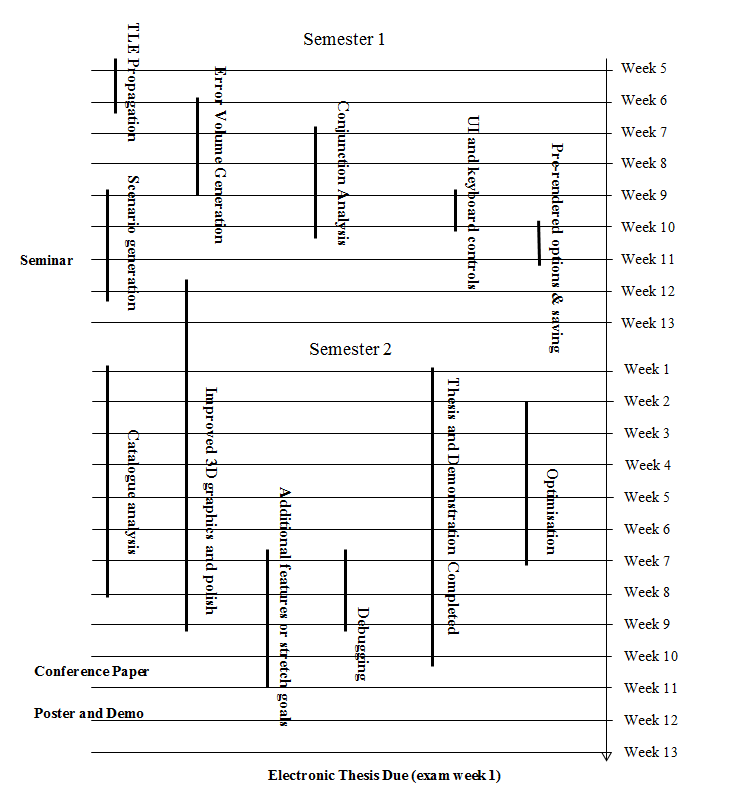
\includegraphics[scale=0.5]{DevSched.png}
			\end{figure}
	
	\section{Possible future work}
	
	There are many areas of possible future work related to this project. Future work directly relating to the implementations in this project would include:
	
	\begin{itemize}
		\item Propagation on a GPU with more memory, allowing for larger real time visualisations
		\item Further optimisations to GPU implementation
		\item UDP implementation with larger buffer size
		\item Parallelise and optimise Unity visualisation to support larger simulations.
		\item Integration of close approach analysis with Unity
		\item Domain decomposition pre-filtering methods to optimise close approach analysis
		\item Further interaction options in Unity visualisation such as selecting objects to retrieve data or performing analysis on selected object.
	\end{itemize}
	
	Areas of further research include: improvements to Two-line element fidelity such as correction methods, further investigation into the utility of Virtual Reality as an investigation/presentation medium (this would include quantifying engagement or learning metrics) and directly comparing the impact of inaccuracy in Gaussian error volumes with Monte-Carlo particle representations in the context of low fidelity threat detection.


	\chapter{Conclusions}
	

	\section{Summary and conclusions}
	
	This project created two visualisation tools and a companion close approach analysis tool using the common TLE/SGP4 approach. It investigated the use of generative Monte-Carlo particles methods and found them to be a useful alternative to the typical Gaussian error volume, particularly when TLE data has aged. \newline 
	
	This investigation further highlights the quick degradation of TLE sets and the need for TLE correction methods, a current area of study (see \cite{tleBIAS, tleCorr}). This investigation found the fidelity afforded by TLE is insufficient to reliably detect close approaches within a threshold of 15km, even close to epoch. A threshold of 25-30km was found to be significantly more reliable. \newline
	
	 Finally, this project found Virtual Reality to be an effective and engaging presentation tool, conferring depth and scale far greater than is possible in other visualisations. Further investigation is needed to quantify these benefits.
	
	
	\appendix
	
	% Chapters after the \appendix command are lettered, not numbered.
	% Setting apart the appendices in the table of contents is awkward:
	
	\addcontentsline{toc}{part}{Appendices}
	\mbox{}
	\newpage
	
	% The \mbox{} command between two \newpage commands gives a blank page.
	% In the contents, the ``Appendices'' heading is shown as being on this
	% blank page, which is the page before the first appendix.  This stops the
	% first appendix from be listed ABOVE the word ``Appendices'' in the
	% table of contents.
	
	% \include appendix chapters here.
	
	\chapter{Code Snippets}
	
	\section{TLE File Handling}
	
	\begin{figure}[H]
		\centering
		\caption{TLE File Handling Code Snippet}
		\label{TLEread}
		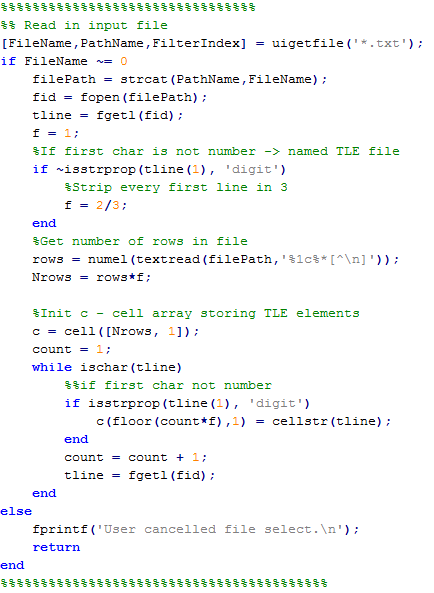
\includegraphics[scale=0.8]{TLEread.png}
	\end{figure}
	
	\begin{figure}[H]
		\centering
		\caption{Particle Generation Code Snippet}
		\label{TLEread}
		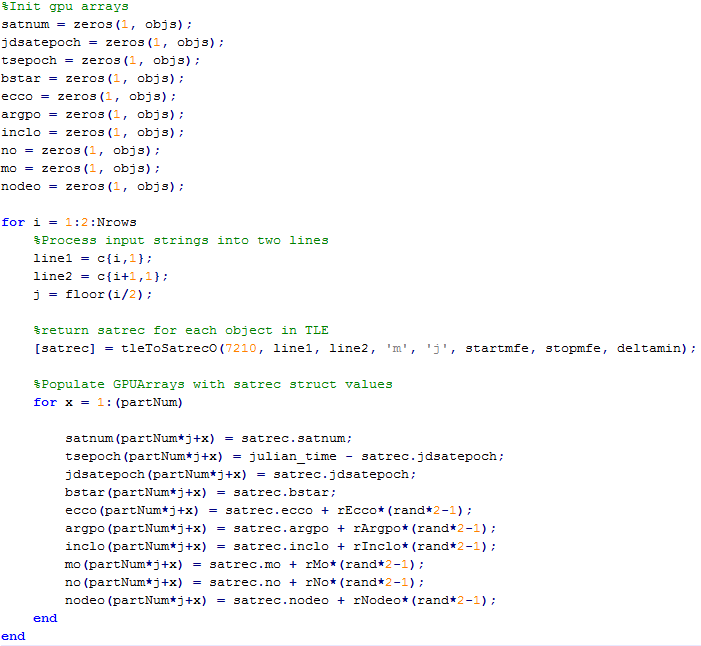
\includegraphics[scale=0.8]{particleToSatrec.png}
	\end{figure}
	
	\begin{figure}[H]
		\centering
		\caption{MATLAB GPU Code Snippet}
		\label{MGPU}
		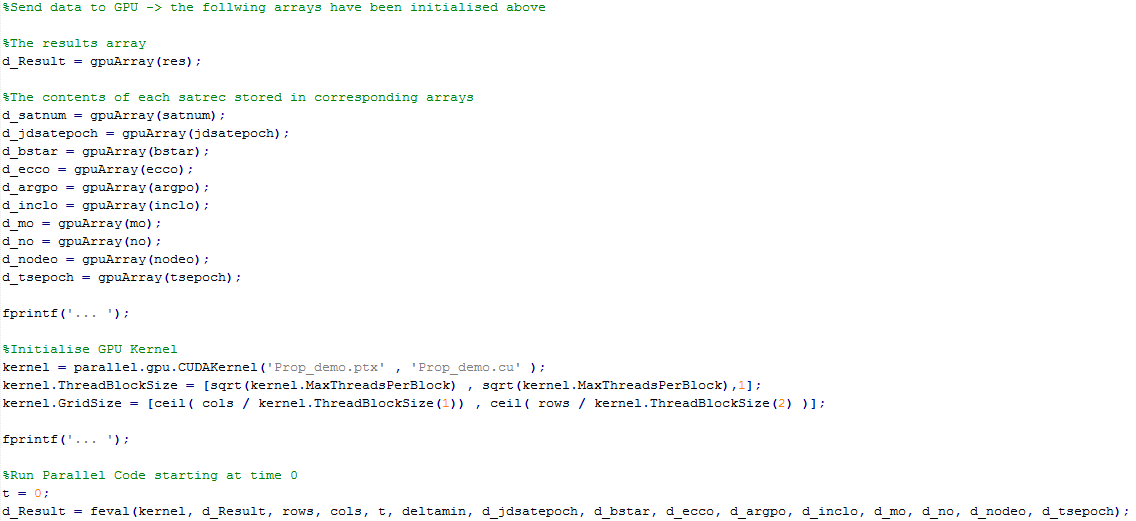
\includegraphics[scale=0.8]{MGPU.png}
	\end{figure}
	
	\begin{figure}[H]
		\centering
		\caption{nVidia CUDA Code Snippet}
		\label{CUDA}
		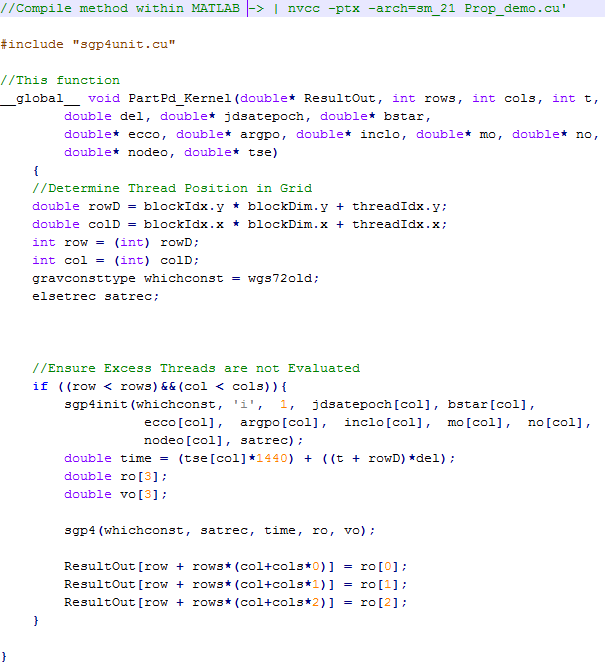
\includegraphics[scale=0.8]{CUDA.png}
	\end{figure}
	
	\begin{figure}[H]
		\centering
		\caption{Unity UDP Decoding Code Snippet}
		\label{uUDP}
		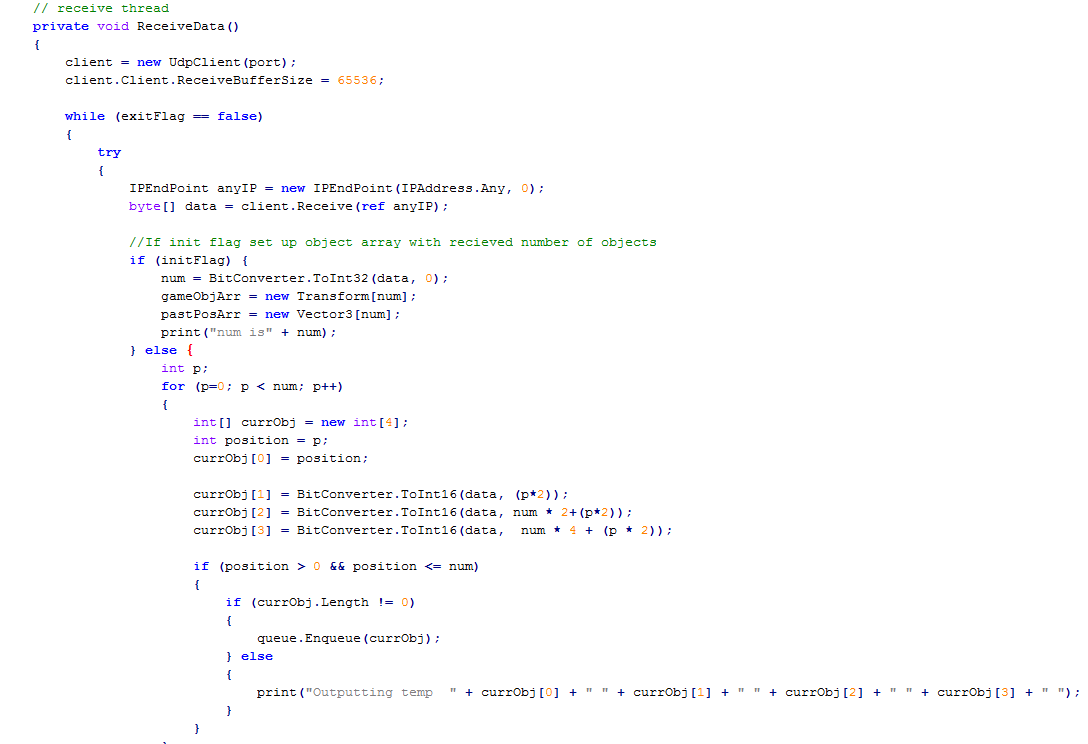
\includegraphics[scale=0.8]{unitySnip.png}
	\end{figure}
	\chapter{Companion Files}
	
	Companion files are provided at the following location (hosted on Dropbox): \newline
	
	\url{https://www.dropbox.com/sh/8jtsg8todazhc81/AACrgWpOaQxdjOygA2Lj2fYLa} \newline
	
	This includes videos of both the MATLAB and Unity Visualisations, all the source MATLAB and Java code and the modified Vallado SGP4 code. \newline
	
	The MATLAB code is compatible with MATLAB R2015b. 
	

	
%	If you wish to make some computer files available to your examiners,
%	you can list and describe the files here.  The files can be supplied
%	on a disk and inserted in a pocket fixed to the inside back cover.
%	
%	The disk will not be needed if you can specify a URL from which the
%	files can be downloaded.
	
	\clearpage
	
	\begin{thebibliography}{99}
		\addcontentsline{toc}{chapter}{Bibliography}
		\bibitem{Allianz}Allianz Global Corporate and Speciality, “Space Risks: A new generation of challenge”, (2012)
		\bibitem{Congress} U.S. Congress, Office of Technology Assessment, “Orbiting Debris: A Space Environmental Problem-Background Paper”, (September 1990), OTA-BP-ISC-72, Washington, DC: U.S. Government Printing Office
		\bibitem{SERC}Space Environment Research Centre, “SERC Partners”, (2014). Retrieved April 1, 2016, URL: \url{http://www.serc.org.au/research/program-3/}
		\bibitem{Kelso}T.S. Kelso, “Analysis of the Iridium 33-Cosmos 2251 Collision”, Centre for Space Standards and Innovation, (2009)
		\bibitem{SpaceTrk3}F. R. Hoots, SpaceTrack Report No.3, Department of Defense, 1980,
		 Retrieved October 1, 2016, URL:\url{https://celestrak.com/NORAD/documentation/spacetrk.pdf}
 		\bibitem{spaceTrack}Science Applications International Corporation, SpaceTrack, Retrieved October 15, 2016, URL:	\url{https://www.space-track.org/}
		\bibitem{SpaceTrk3R}D. A. Vallado, Revisiting Spacetrack Report No.3, Centre for Space Standards and Innovation, Colorado Springs, 2006, Retrieved October 1, 2016, URL: \url{https://celestrak.com/publications/AIAA/2006-6753/AIAA-2006-6753.pdf}
		\bibitem{Hobson}Hobson, T.,  Sensor Management for Enhanced Catalogue Management of Resident Space Objects, 2014, University of Queensland, p146.
		\bibitem{NASAtle} Kim Dismukes, Two-line Element Definition, 2011, NASA, Retrieved October 1, 2016, URL: \url{http://spaceflight.nasa.gov/realdata/sightings/SSapplications/Post/JavaSSOP/SSOP_Help/tle_def.html}
		\bibitem{Ghrist}R.W. Ghrist ,D. Plakalovic, “Impact of Non-Gaussian Error Volumes on Conjunction Assessment Risk Analysis”, (2012), a.i. Solutions, Inc., Colorado Springs, CO 80915
		\bibitem{Jiajun}Y Jianjun, Z Jianqiu, Z Zesen, “Gaussian Sum PHD Filtering Algorithm for Nonlinear Non-Gaussian Model”, (2008), Department of Electronic Engineering, Fudan University, Shanghai 200433, China
		\bibitem{Terajanu}G. Terejanu, P. Singlay, T. Singhz, P.D. Scottx, “Uncertainty Propagation for Nonlinear Dynamical Systems using Gaussian Mixture Models, (2008), American Institute of Aeronautics and Astronautics
		\bibitem{heights}A. A. Suárez, "Virtual Reality: A tool for treating phobias of heights", 2013, University of Turabo, Eleventh LACCEI Latin American and Caribbean Conference for Engineering and Technology
		\bibitem{tele}A. Biagioli, HTC Vive Teleportation System with Parabolic Pointer, 2016, Retrieved October 1, 2016, URL: \url{https://github.com/Flafla2/Vive-Teleporter}
		\bibitem{agiAcc}AGI, Conjunction Analysis Toolkit, 2016,  \url{http://www.agi.com/resources/help/online/stk/11.0/Content/cat/Cat02-04.htm}
		\bibitem{agiTLEAcc}D. L. Oltrogge, J. Ramrath, Parametric Characterization of SGP4 Theory and TLE Positional Accuracy, AGI, 2014, Retrieved October 5, 2016, URL:		\url{https://www.agi.com/downloads/resources/white-papers/20140911_EGP_Fit_Capability_AMOS_3317135_v04.docx.pdf}
		\bibitem{accTLE}J. Mason, Development of a MATLAB/STK TLE Accuracy Assessment Tool, International Space University, 2009, Retrieved October 15, 2016, URL:		\url{https://arxiv.org/ftp/arxiv/papers/1304/1304.0842.pdf}
		\bibitem{tleBIAS}J. C. Bennett, Improving low-Earth orbit predictions using two-line element data with bias correction, 	
		The Satellite Positioning for Atmosphere, Climate and Environment (SPACE) Research Centre,
		School of Mathematical and Geospatial Sciences, 2012, Retrieved October 15, 2016, URL:		\url{http://www.amostech.com/technicalpapers/2012/astrodynamics/bennett.pdf}
		\bibitem{tleCorr}W. Lui.  ,R. Wang ,R. Yan ,J. Gong, Improving LEO prediction precision with TLEs, Center for Space Science and Applied Research, 2013, Retrieved October 15, 2016, URL:		\url{http://aero.tamu.edu/sites/default/files/faculty/alfriend/CTI2P/CT3%20S2.3%20Liu.pdf}

		
		%			[9] , 
		%			[10] - 
		
%			[1] - 
%			[2] - 
%			[3] - NASA Orbital Debris Program Office, “Orbital debris – Graphics”, (2009, July). , Accessed April 1, 2016, URL: http://orbitaldebris.jsc.nasa.gov/photogallery/beehives.html
%			[4] - 
%			[5] 
%			[6] – V.T. Coppola, S. Dupont, K. Ring, F. Stoner, “Accessing Satellite Conjunctions for the Entire Space Catalogue  using COTS Multi-core Processor Hardware”, (2014)
%			[7] – S. Alfano,  “Review of Conjunction Probability Methods for Short-term Encounters”, (2013), American Institute of Aeronautics and Astronautics 
%			
%			[11] – T. Hobson, - “Sensor Management for Enhanced Catalogue Maintenance of Resident Space Objects”, (2014), The University of Queensland, Section 6.2
%			[12] – X. Xu, Y. Xiong, “A Method for Calculating Collision Probability between Space Objects”, (2013)
%			[13] – R. Hall, Dr. S. Alfano, A. Ocampo, “Advances in Satellite Conjunction Analysis”, (2010)
%			[14] - D.A. Vallado, “Fundamentals of Astrodynamics”, (2007) Third Edition, Microcosm Press, Hawthorne, CA, and Springer, New York, NY. 
%			[15] D.A. Vallado, P Crawford, “SGP4 Orbit Determination”, (2008), Center for Space Standards and Innovation, Colorado Springs, Colorado, 80920
%			[16] CelestTrak, “FAQ: Two-Line Element Set Format”, Retrieved April 4th, 2016, URL: https://celestrak.com/columns/v04n03/
%			[17] AGI, “AGI Software for SSA”, (2014), White Paper
%			[18] Scitor Corporation, “Space Track Data Catalogue”, Retrieved April 5th, 2016, URL: https://www.space-track.org/
			
		
	\end{thebibliography}
	
\end{document}